\chapter{Results}
\label{chapter:results}
Having described the implementation of all the models introduced in \autoref{chapter:volatility} and the calibration and interpolation methods referenced in \autoref{chapter:implementation}, in this chapter we study the results of the calibration and compare all the models and respective simulations.

We will calibrate the SABR and Heston models' parameters with a dataset of implied volatilities for European options with different maturities and strike prices. This data is shown in \autoref{chapter:mktdata}. As stated before, the closed form solutions will be used in this calibration procedure. After the calibration, we are able to produce a function from these closed-form solutions that relates the strike price with the implied volatility, using the models' calibrated parameters. This function - henceforth named \emph{theoretical function} - should, in principle, closely fit the implied volatility data.

To validate the SABR and Heston models' closed-form solutions, after finding the optimal parameters with the calibration procedure, we will input them into a Monte Carlo pricer, adapted to each model, and calculate the simulated option prices of each calibrated model. This price will then be converted into an implied volatility (using eq.\eqref{impvolform}) for the simulation to be comparable to the data and the theoretical function. To better grasp the behavior of the simulations we will repeat them a large number of times, $N_{\mathrm{reps}}$, averaging the results to produce a function also relating the strike price with the implied volatility - henceforth named \emph{simulated function} -  and extracting from them the 95\% confidence bands of the simulations - these confidence bands are obtained by sorting the simulated implied volatilities for each strike, and then extracting both the 97.5\% highest and the 2.5\% lowest, using these values as the upper and lower bounds of the confidence bands, so that 95\% of all observations are contained between them.



As for Dupire's local volatility data, the required Delaunay triangulation introduced in \autoref{section:Surface Interpolation (Dupire)} will be performed on the aforementioned data. The resulting interpolation will be used to obtain the local volatility surface, which will be input into a Monte Carlo pricer to generate the option price under this model's assumptions. As done for the Heston and SABR models, we will run this pricer a large number of times, $N_{\mathrm{reps}}$, to obtain the average simulated function and the 95\% confidence bands. Because no closed-form solutions exist for this model, no theoretical functions will be displayed in this case.


For the models to be comparable, we need to make sure that the same global parameters are used in all the adjustments and simulations, namely the initial stock price, $S_0$, the risk-free interest rate, $r$, the number of Monte Carlo pricer repetitions (to be averaged, producing the expected simulated function and the confidence bands), $N_{\mathrm{reps}}$, and the time step size and the number of paths simulated, $\Delta t$ and $N_{\mathrm{paths}}$, both used in the Monte Carlo simulations. Their values are shown in \autoref{tab:defaultparam}.
\begin{table}[H]
    \centering
        \renewcommand{\arraystretch}{0.8}
\begin{tabular}{@{}lcccr@{}}
\toprule
$S_0$($\EUR$) & $r$($\SI{}{\per\year}$) & $\Delta t$(days) & $N_{\mathrm{paths}}$ & $N_{\mathrm{reps}}$ \\ \midrule
1 & 0 & 0.5 & 100 000 & 100\\
\bottomrule
\end{tabular}
  \caption[Global parameters used throughout all simulations.]{Global parameters used throughout all simulations.}
  \label{tab:defaultparam}
\end{table}


The Monte Carlo pricers of each model will then be modified to price Barrier options instead of the European options used in the calibration. These results will be studied with some detail but, due to a lack of real market data, there is no way to corroborate their validity.

As a side note, we should also point out that for the maturities we used the typical market convention of defining a month as having only 21 days, to account only for the days when exchanges are open. Thus, we assume that a year has 252 (open market) days.


\section{Constant Volatility Model}
To find how well our models perform, we need some reference against which to compare them. One clear possibility is to assume a constant volatility throughout the options' duration, since this is the simplest possible case - any other model should be able to outperform this one.

The equation that generates each stock price path is therefore given by
\begin{equation}
dS(t)=rS(t)dt+\sigma S(t)dW(t).
\end{equation}

With this constant volatility model, we can choose to fit the datasets with different maturities independently of one another or together as an ensemble. In other words, we can do several independent fits, one for each maturity, or a single ensemble fit, for all maturities together. The former will be useful when benchmarking the Static SABR model, since for that model the adjustments will also be performed independently (Static SABR performs badly for multiple maturities). The latter will be more appropriate when studying the remaining models - Dupire, Heston and Dynamic SABR - since these fit the whole implied volatility surface (i.e. multiple maturities together). Thus, both versions will be implemented and briefly studied. To clarify, we will still represent all maturities for both adjustment types (independent/dependent), but in the independent case the fits will be done independently for each maturity - a different (constant) implied volatility will be fitted for each maturity - and in the dependent case a single implied volatility will be fitted to the whole ensemble.

\vfill
\newpage

\subsection{Independent Fits}
We begin by presenting the results of fitting a constant volatility function to the sets of data with different maturities \emph{independently}.


In \autoref{fig:ConstVol} we show the plots of each fitted implied volatility curve - the \emph{theoretical functions} - along with the provided market data. We also present the results of the Monte Carlo pricer - the \emph{simulated functions} - and the simulations' confidence bands.
\begin{figure}[H]
  \begin{subfigmatrix}{2}
    \subfigure[$T=21$ days]{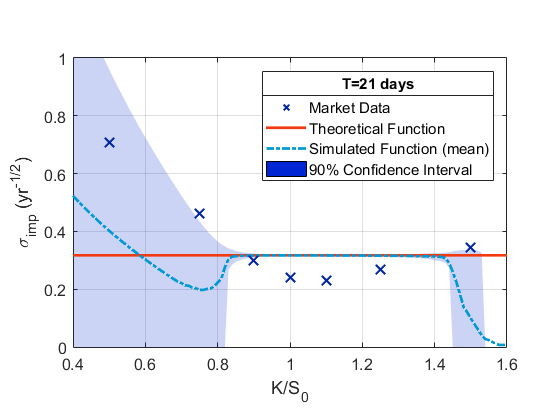
\includegraphics[width=0.49\linewidth,trim={0.25cm 0.45cm 1.1cm 1.4cm},clip]{ConstVol1.png}}
    \subfigure[$T=42$ days]{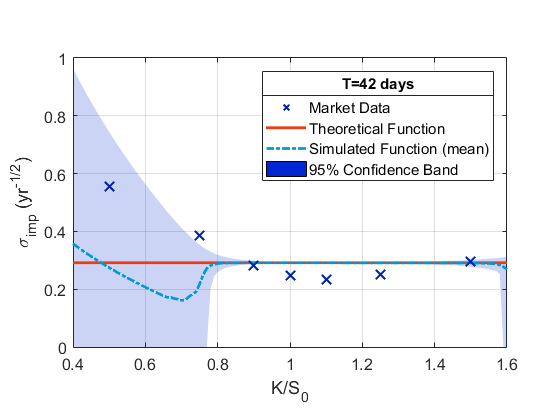
\includegraphics[width=0.49\linewidth,trim={0.25cm 0.45cm 1.1cm 1.4cm},clip]{ConstVol2.png}}
    \subfigure[$T=63$ days]{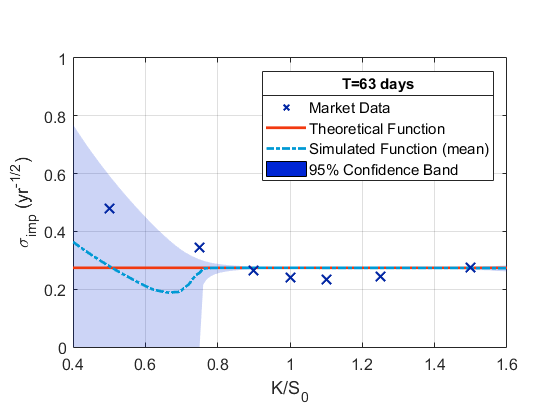
\includegraphics[width=0.49\linewidth,trim={0.25cm 0.45cm 1.1cm 1.4cm},clip]{ConstVol3.png}}
    \subfigure[$T=126$ days]{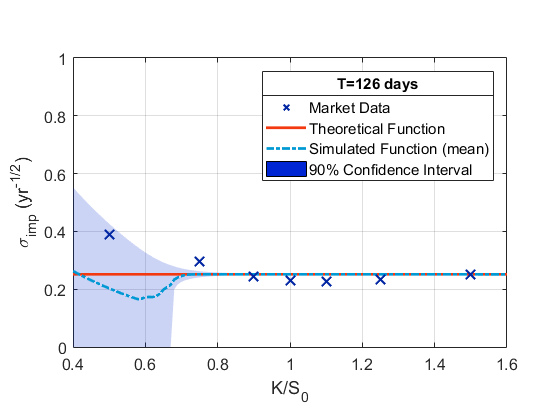
\includegraphics[width=0.49\linewidth,trim={0.25cm 0.45cm 1.1cm 1.4cm},clip]{ConstVol4.png}}
  \end{subfigmatrix}
  \caption[Implied volatility functions fitted independently to the implied volatility data for different maturities under constant volatility model, plotted with their respective Monte Carlo simulated functions along with their 95\% confidence bands.]{Implied volatility functions (red lines) fitted \emph{independently} to the implied volatility data (crosses) for different maturities under constant volatility model, plotted with their respective Monte Carlo simulated functions (light-blue dot-dashed lines) along with their 95\% confidence bands (blue region).}
  \label{fig:ConstVol}
\end{figure}

\vfill
\newpage

The fitted parameter, which, in this case, is only the constant implied volatility, is presented in \autoref{tab:ConstVolPar} for each of the maturities, along with the respective cost function's value (eq.\eqref{cost}).

\begin{table}[H]
    \centering
        \renewcommand{\arraystretch}{0.8}
\begin{tabular}{@{}lcr@{}}
\toprule
$T$ (days) & $\sigma_{imp,\mathrm{mdl}}$ ($\SI{}{\year\tothe{-1/2}}$) & Cost \\ \midrule
21 & 0.3174 & 0.0635 \\
42 & 0.2918 & 0.0282 \\
63 & 0.2742 & 0.0164 \\
126& 0.2518 & 0.0069 \\
\bottomrule
\end{tabular}
  \caption[Fitted implied volatilities for each maturity (fitted independently) under constant volatility model.]{Fitted implied volatilities for each maturity (fitted independently) under constant volatility model.}
  \label{tab:ConstVolPar}
\end{table}


By observing the fit results in \autoref{tab:ConstVolPar} we see that the cost function decreases with the maturity. This is indeed what is expected, since the implied volatility surface becomes flatter as maturity increases, as can be seen from the market data (and also as we can see in \autoref{fig:realimpliedvol}). This makes the constant volatility function a better approximation in such cases, which decreases the cost function's value.

We should note that the fitted constant implied volatilities' values are typical for what is usually observed in the market, i.e. values around $0.25\SI{}{\year\tothe{-1/2}}$.

One other property that we can observe is that the constant implied volatility also decreases with maturity. The reason behind this is the simple fact that earlier maturities contain higher implied volatilities (for the strikes far from $S_0$), which pull the fitted constant volatility function upwards.


We now focus on the results presented in \autoref{fig:ConstVol}.
First, we can see that the theoretical functions (full red lines) clearly don't represent the market data. This is indeed what is expected, since the constant volatility model doesn't cover the volatility smile phenomenon, which we explained before.

Secondly, by comparing the theoretical and simulated functions, we must note that the simulation performs extremely well for strikes near $S_0$. Notice that the simulated function (dot-dashed blue line) perfectly follows the constant volatility theoretical result (full red line) in this region, and that the confidence bands converge to the simulated function indicating that all simulations produced the same result. This seems to suggest that the simulation is working as expected for this particular region.

Thirdly, we notice that on the earliest maturity (i.e. 21 days), for strikes much larger than $S_0$ (e.g. $K/S_0=1.5$), the simulated implied volatilities go to zero, even though they should remain constant. The reason behind this has already been discussed in \autoref{subsection:Pricing options from simulations} and relates to the very, very small number of paths that reach such high strikes and end up contributing to the option price (which is then converted to an implied volatility). For the case of strike $K/S_0=1.5$, and maturity $T=21$ days, under this constant volatility model the number of paths that reach the strike is indeed approximately $0.25$ out of $100\,000$ (i.e. one out of four Monte Carlo simulations of $100\,000$ paths contains a single path that is able to reach such a high strike). This problem is not observed on the remaining maturities for the simple reason that, because they are given more time to evolve, more paths are able to reach these high strikes and contribute to the option price.
To solve this problem, we could significantly increase the number of simulations, so that the number of paths that are able to reach these high strikes is enough to produce a good estimate of the option price. The problem with this solution is the very significant increase in the computation time required, which makes it impractical.
If we lowered the number of simulated paths from $100\,000$ to any other smaller amount, the problem described before would become even more severe, and the later maturities would eventually also display the problem observed in the earliest maturity.

Finally, we must discuss the large confidence bands for strikes much lower than $S_0$ (e.g. $K/S_0=0.5$), occurring over all maturities. To explain this, we require the points made in \autoref{section:vega}, particularly for \autoref{fig:Vega2}, where we introduced the concept of \emph{relative change} of the option price w.r.t. the volatility. Repeating the example from before, a relative change of $5$ means that a variation of $1\%$ in the volatility will produce a variation of $5\%$ in the option price. We saw that for low strikes, this quantity was extremely small. This means that the option price is very insensitive to the volatility (i.e. a change in the volatility barely affects the price), but it also means that the volatility is very sensitive to the option price (i.e. a small change in the price significantly affects its implied volatility). The reason why this observation is important here is because we are calculating option prices from simulations and then converting them to implied volatilities (solving eq.\eqref{impvolform}).
Even though the Monte Carlo pricer is expected to produce a very good estimation of option prices with lower strikes (a very large number of paths contribute to the option price, so the estimation will be very accurate, with very little variation - the opposite of what we described before for high strikes), because there will always be \emph{some} variation on different simulations, the pricer is expected to produce some very slightly different results when executed multiple times, which is enough to cause some of the generated implied volatilities to differ significantly from one another, some going to approximately zero others increasing significantly, which explains the large confidence bands. This is not observed in the higher strikes because the value of relative change is very small. Furthermore, in the low strike regions, we can see that the confidence bands seem to decrease in size for the higher maturities. This phenomenon was also expected from the conclusions made in \autoref{fig:Vega2}, where we noted that the relative change decreased with the maturity, which attenuates the severity of the problem posed before.

These two last problems are not only applicable to the constant volatility model and will also be observed in all the other models, as we shall see next.

\vfill
\newpage

In \autoref{tab:CV} we show the values of the implied volatilities fitted to the data for the different maturities, along with their relative errors when compared to the provided implied volatility data, shown in \autoref{tab:mktdata}. We also show the respective European option prices of said fitted volatilities and their corresponding relative errors (when compared to the option prices of the provided data, also in \autoref{tab:mktdata}).



\begin{table}[H]
\centering
\renewcommand{\arraystretch}{0.8}
\begin{tabular}{@{}cccrcr@{}}
\toprule
$T$(days) & $K/S_0$ & $\sigma_{imp,\mathrm{mdl}}$($\SI{}{\year\tothe{-1/2}}$) & $\mathrm{Error}_{\sigma}(\%)$ & $C_{\mathrm{mdl}}$($\EUR$) & $\mathrm{Error}_{C}(\%)$ \\ \midrule
\multirow{7}{*}{21} & 0.50 & \multirow{7}{*}{0.3174}& 55 & \num{5.000E-01} & 0 \\
 & 0.75 &  & 31 & \num{2.500E-01} & 0 \\
 & 0.90 &  & 6 & \num{1.054E-01} & 1 \\
 & 1.00 &  & 31 & \num{3.654E-02} & 31 \\
 & 1.10 &  & 37 & \num{7.406E-03} & 206 \\
 & 1.25 &  & 18 & \num{2.501E-04} & 368 \\
 & 1.50 &  & 8 & \num{1.119E-07} & 81 \\ \midrule
\multirow{7}{*}{42} & 0.50 & \multirow{7}{*}{0.2918} & 47 & \num{5.000E-01} & 0 \\
 & 0.75 &  & 25 & \num{2.503E-01} & 1 \\
 & 0.90 &  & 3 & \num{1.117E-01} & 1 \\
 & 1.00 &  & 19 & \num{4.749E-02} & 19 \\
 & 1.10 &  & 24 & \num{1.500E-02} & 76 \\
 & 1.25 &  & 16 & \num{1.575E-03} & 154 \\
 & 1.50 &  & 2 & \num{1.244E-05} & 21 \\ \midrule
\multirow{7}{*}{63} & 0.50 & \multirow{7}{*}{0.2742} & 43 & \num{5.000E-01} & 0 \\
 & 0.75 &  & 21 & \num{2.508E-01} & 1 \\
 & 0.90 &  & 3 & \num{1.165E-01} & 1 \\
 & 1.00 &  & 14 & \num{5.465E-02} & 14 \\
 & 1.10 &  & 18 & \num{2.069E-02} & 46 \\
 & 1.25 &  & 12 & \num{3.331E-03} & 85 \\
 & 1.50 &  & 0 & \num{7.437E-05} & 3 \\ \midrule
\multirow{7}{*}{126} & 0.50 & \multirow{7}{*}{0.2518} & 35 & \num{5.000E-01} & 0 \\
 & 0.75 &  & 15 & \num{2.534E-01} & 1 \\
 & 0.90 &  & 3 & \num{1.288E-01} & 1 \\
 & 1.00 &  & 10 & \num{7.094E-02} & 10 \\
 & 1.10 &  & 11 & \num{3.488E-02} & 22 \\
 & 1.25 &  & 8 & \num{9.977E-03} & 32 \\
 & 1.50 &  & 0 & \num{8.510E-04} & 1 \\ \bottomrule
\end{tabular}
  \caption[Fitted implied volatilities (fitted independently) and respective option prices along with their corresponding relative errors w.r.t. the provided data under the constant volatility model.]{Fitted implied volatilities (fitted independently) and respective option prices along with their corresponding relative errors w.r.t. the provided data under the constant volatility model.}
  \label{tab:CV}
\end{table}

One interesting property that we can extract from the data in \autoref{tab:CV} is that the relative errors of the option prices, $\mathrm{Error}_{C}$, seem to increase with the strike. This is indeed expected from the conclusions obtained in \autoref{section:vega}: we saw that options with high strikes had a higher relative change on the option price w.r.t. the volatility. This means that a small (relative) variation in the implied volatility causes a very considerable (relative) change in the option price. Observing, for example, the data for the strike $K/S_0=1.25$ and the maturity $T=21$ days, we see that even though the relative error for the implied volatility is only $18\%$, the resulting relative error on the option price is $368\%$, which is a staggering difference. On the other hand, we also saw that for options with low strikes the value of relative change was small, which means that even large (relative) changes in the implied volatility barely affect the price. Observing now, for example, the data for the strike $K/S_0=0.75$ on the same maturity, the relative error on the implied volatility is $55\%$, significantly higher than before, but the respective relative error on the option price is $0\%$ (rounded off to the units).

Furthermore, we noted in \autoref{section:vega} that the value of relative change for strikes $K/S_0=1$ was approximately $1$ throughout all maturities. This would mean that for such strikes, the relative errors in the implied volatility would be approximately the same as the relative errors in the option price, which is precisely verified in the data throughout all maturities (see, for example, the relative errors of $14\%$ in both the implied volatility and option price for the maturity $T=63$ days and strike $K/S_0=1$).

Finally, it is clear that the relative errors of the option price decrease with the maturity (e.g. for the maturity of 21 days we have errors up to $368\%$, whereas for the maturity of 63 days they only go up to $85\%$). This phenomenon was also expected from the conclusions made before, where we noted that the relative change decreased with maturity, which attenuates the high relative change phenomenon.

We can thus conclude that the results corroborate what would be expected from our predictions.

\vfill
\newpage

\subsection{Dependent Fits}
We now present the results obtained from fitting constant volatility function to the ensemble with all implied volatility data, regardless of maturity.

In \autoref{fig:ConstVol2} we show the theoretical and simulated functions as well as the provided market data.
\begin{figure}[H]
  \begin{subfigmatrix}{2}
    \subfigure[$T=21$ days]{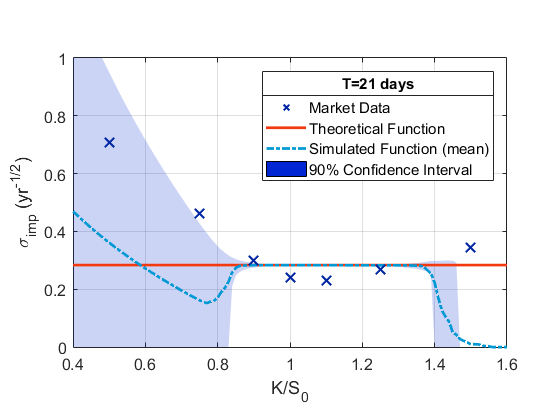
\includegraphics[width=0.49\linewidth,trim={0.25cm 0.45cm 1.1cm 1.4cm},clip]{ConstVol12.png}}
    \subfigure[$T=42$ days]{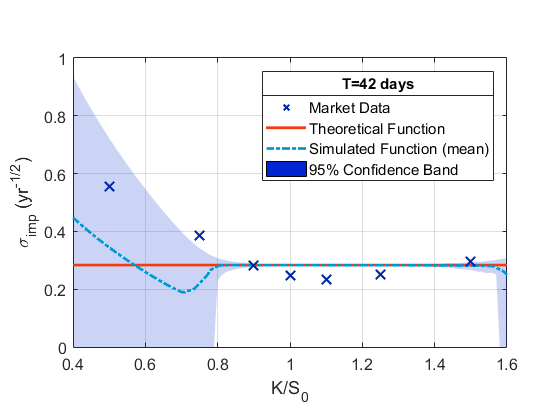
\includegraphics[width=0.49\linewidth,trim={0.25cm 0.45cm 1.1cm 1.4cm},clip]{ConstVol22.png}}
    \subfigure[$T=63$ days]{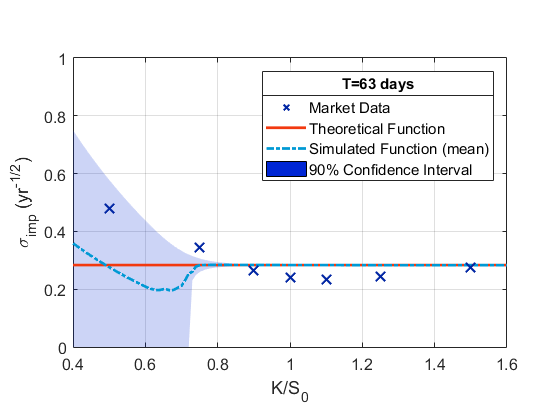
\includegraphics[width=0.49\linewidth,trim={0.25cm 0.45cm 1.1cm 1.4cm},clip]{ConstVol32.png}}
    \subfigure[$T=126$ days]{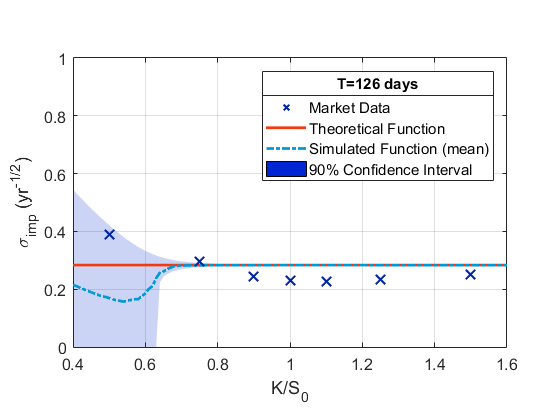
\includegraphics[width=0.49\linewidth,trim={0.25cm 0.45cm 1.1cm 1.4cm},clip]{ConstVol42.png}}
  \end{subfigmatrix}
  \caption[Implied volatility functions fitted simultaneously to the implied volatility data for different maturities under constant volatility model, plotted with their respective Monte Carlo simulated functions along with their 95\% confidence bands.]{Implied volatility functions (red lines) fitted \emph{simultaneously} to the implied volatility data (crosses) for different maturities under constant volatility model, plotted with their respective Monte Carlo simulated functions (light-blue dot-dashed lines) along with their 95\% confidence bands (blue region).}
  \label{fig:ConstVol2}
\end{figure}

The fitted implied volatility is represented in \autoref{tab:ConstVolPar2} as well as the cost function's value.
\begin{table}[H]
    \centering
        \renewcommand{\arraystretch}{0.8}
\begin{tabular}{@{}lr@{}}
\toprule
 $\sigma_{imp,\mathrm{mdl}}$ ($\SI{}{\year\tothe{-1/2}}$) & Cost \\ \midrule
0.2838 & 0.1248 \\
\bottomrule
\end{tabular}
  \caption[Fitted implied volatility for all maturities (fitted simultaneously) under constant volatility model.]{Fitted implied volatility for all maturities (fitted simultaneously) under constant volatility model.}
  \label{tab:ConstVolPar2}
\end{table}


\iffalse
First, when we compare the implied volatility fitted to all the maturities with the results of the independent fits (in \autoref{tab:ConstVolPar}) we see that the former is actually the average of the latter. \hl{why?}
\fi


Regarding the plots in \autoref{fig:ConstVol2} they look very similar to those in \autoref{fig:ConstVol}, so not much more can be added regarding their analysis.


As before, we now show the fitted implied volatility and its corresponding option prices as well as their relative errors when compared against the data in \autoref{tab:mktdata}.

\begin{table}[H]
\centering
\renewcommand{\arraystretch}{0.8}
\begin{tabular}{@{}cccrcr@{}}
\toprule
$T$(days) & $K/S_0$ & $\sigma_{imp,\mathrm{mdl}}$($\SI{}{\year\tothe{-1/2}}$) & $\mathrm{Error}_{\sigma}(\%)$ & $C_{\mathrm{mdl}}$($\EUR$) & $\mathrm{Error}_{C}(\%)$ \\ \midrule
\multirow{7}{*}{21} & 0.50 & \multirow{7}{*}{0.2838} & 60 & \num{5.000E-01} & 0 \\
 & 0.75 &  & 39 & \num{2.500E-01} & 0 \\
 & 0.90 &  & 5 & \num{1.036E-01} & 1 \\
 & 1.00 &  & 17 & \num{3.267E-02} & 17 \\
 & 1.10 &  & 23 & \num{5.191E-03} & 114 \\
 & 1.25 &  & 5 & \num{8.977E-05} & 68 \\
 & 1.50 &  & 17 & \num{7.031E-09} & 99 \\ \midrule
\multirow{7}{*}{42} & 0.50 & \multirow{7}{*}{0.2838} & 49 & \num{5.000E-01} & 0 \\
 & 0.75 &  & 27 & \num{2.502E-01} & 1 \\
 & 0.90 &  & 1 & \num{1.108E-01} & 0 \\
 & 1.00 &  & 15 & \num{4.620E-02} & 15 \\
 & 1.10 &  & 21 & \num{1.402E-02} & 64 \\
 & 1.25 &  & 12 & \num{1.336E-03} & 115 \\
 & 1.50 &  & 4 & \num{8.299E-06} & 48 \\ \midrule
\multirow{7}{*}{63} & 0.50 & \multirow{7}{*}{0.2838} & 41 & \num{5.000E-01} & 0 \\
 & 0.75 &  & 18 & \num{2.510E-01} & 1 \\
 & 0.90 &  & 7 & \num{1.179E-01} & 2 \\
 & 1.00 &  & 18 & \num{5.656E-02} & 18 \\
 & 1.10 &  & 22 & \num{2.227E-02} & 57 \\
 & 1.25 &  & 16 & \num{3.925E-03} & 118 \\
 & 1.50 &  & 3 & \num{1.087E-04} & 42 \\ \midrule
\multirow{7}{*}{126} & 0.50 & \multirow{7}{*}{0.2838} & 27 & \num{5.000E-01} & 0 \\
 & 0.75 &  & 4 & \num{2.559E-01} & 0 \\
 & 0.90 &  & 16 & \num{1.361E-01} & 7 \\
 & 1.00 &  & 24 & \num{7.992E-02} & 24 \\
 & 1.10 &  & 25 & \num{4.317E-02} & 51 \\
 & 1.25 &  & 21 & \num{1.499E-02} & 98 \\
 & 1.50 &  & 13 & \num{1.967E-03} & 129 \\ \bottomrule
\end{tabular}
  \caption[Fitted implied volatilities (fitted simultaneously) and respective option prices along with their corresponding relative errors w.r.t. the provided data under the constant volatility model.]{Fitted implied volatilities (fitted simultaneously) and respective option prices along with their corresponding relative errors w.r.t. the provided data under the constant volatility model.}
  \label{tab:CV2}
\end{table}

As before, the relative errors of the option prices seem to increase with the strike, even though the same behavior is not observed for the relative errors of the implied volatilities, which has already been discussed.

\vfill
\newpage

\section{Dupire Model}
\label{section:Dupire Model}
The stochastic differential equation for the stock price paths under the local volatility model was hypothesized to be given by
\begin{equation}\label{dupmodds}
dS(t)=rS(t)dt+\sigma(S(t),t)S(t)dW(t),
\end{equation}
\noindent where $\sigma(S(t),t)$ can be obtained through Dupire's model, defined in \autoref{subsection:Dupire}, which is given by
\begin{equation}\label{dupmodds2}
\sigma(S(t),t)=\sqrt{\frac{\displaystyle\sigma_{imp}^2+2t\sigma_{imp}\pdv{\sigma_{imp}}{T}+2r(S(t))t\sigma_{imp}\pdv{\sigma_{imp}}{K}}{\displaystyle\left(1+(S(t))d_1\sqrt{t}\pdv{\sigma_{imp}}{K}\right)^2+(S(t))^2t\sigma_{imp}\left(\pdv{^2\sigma_{imp}}{K^2}-d_1\left(\pdv{\sigma_{imp}}{K}\right)^2\sqrt{t}\right)}},
\end{equation}
\noindent where $d_1$ is defined as
\begin{equation}
d_1=\frac{\log(S_0/S(t))+\left(r+\frac{1}{2}\sigma_{imp}^2\right)t}{\sigma_{imp}\sqrt{t}}.
\end{equation}

As we mentioned in \autoref{section:Surface Interpolation (Dupire)}, we must produce the implied volatility surface from the market data using an interpolation algorithm. Applying the Delaunay triangulation defined earlier, we obtain the implied volatility surface, shown in \autoref{fig:DupImpV} along with its contour plot.
From this surface we can easily extract (numerically) the gradients required for the local volatility formula.



\begin{figure}[H]
  \begin{subfigmatrix}{2}
    \subfigure[$\sigma_{imp}$ surface]{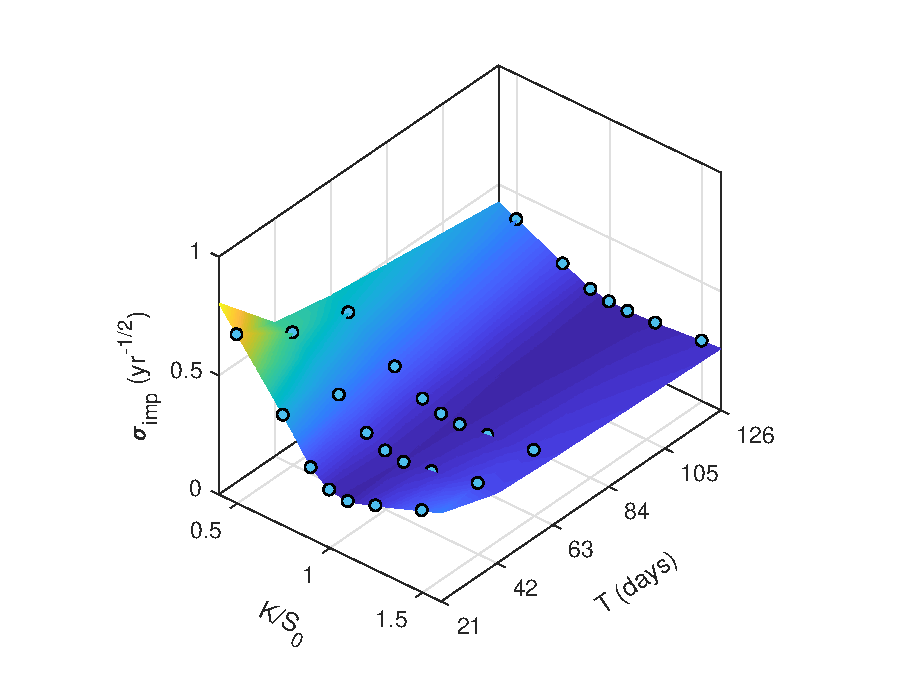
\includegraphics[width=0.49\linewidth,trim={1.7cm 0.45cm 2.cm 0.85cm},clip]{ImpliedV.eps}}
    \subfigure[$\sigma_{imp}$ contour plot]{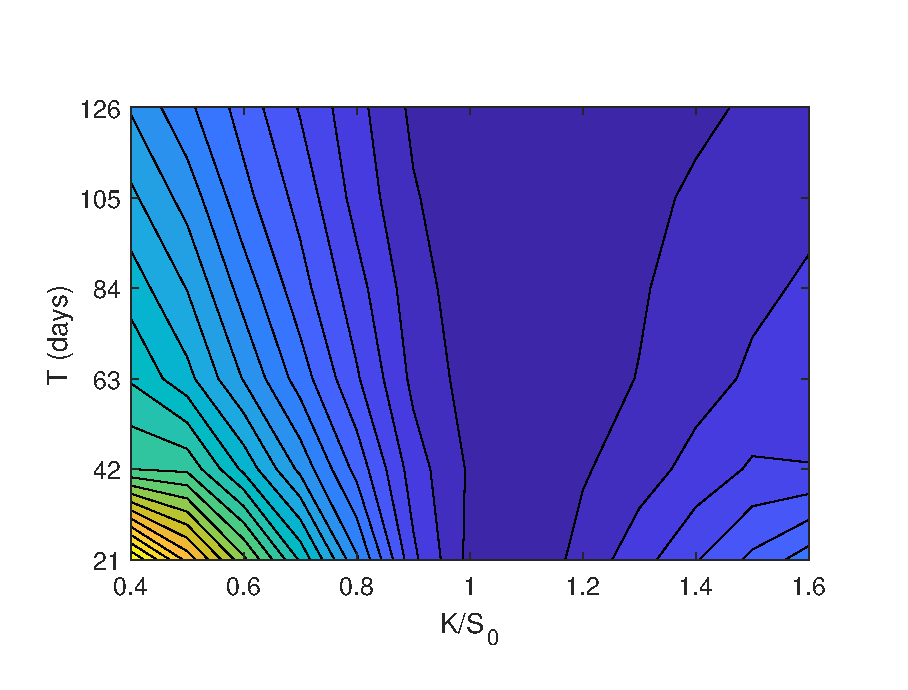
\includegraphics[width=0.49\linewidth,trim={0.2cm 0.5cm 1.25cm 1.55cm},clip]{ImpliedVC.eps}}
  \end{subfigmatrix}
    \caption[Implied volatility surface and corresponding contour plot of the function interpolated linearly between the original data points using Delaunay triangulation.]{Implied volatility surface (left) and corresponding contour plot (right) of the function interpolated linearly between the original data points (blue circles) using Delaunay triangulation.}\label{fig:DupImpV}
\end{figure}   


Observing this interpolated surface, we see that its curvature decreases with maturity - the volatility smile becomes less prominent for later maturities - which can also be observed in the provided data, shown in \autoref{chapter:mktdata}.

As we stated before in \autoref{section:Surface Interpolation (Dupire)}, from the implied volatility surface we should generate a grid of local volatilities, from which we will obtain the local volatility surface. This grid was obtained by defining some limits on the strike prices and maturities, with $K_{min}$ and $K_{max}$ being the smallest and largest strikes in the grid, with intervals $\Delta K$ between the them, and with $T_{min}$ and $T_{max}$ being the smallest and largest maturities, with intervals $\Delta T$. The values for these quantities that we used throughout this section are shown in \autoref{tab:DupR}.


\begin{table}[H]
    \centering
        \renewcommand{\arraystretch}{0.8}
\begin{tabular}{@{}cccccc@{}}
\toprule
$T_{min}$(days) & $T_{max}$(days) & $\Delta T$(days) & $K_{min}/S_0$ & $K_{max}/S_0$ & \multicolumn{1}{c}{$\Delta K/S_0$}\\ \midrule
21 & 126 & 10.5 & 0.4 & 1.6 & \multicolumn{1}{c}{0.05} \\ \bottomrule
\end{tabular}
  \caption[Parameters used in the interpolation section of Dupire's model.]{Parameters used in the interpolation section of Dupire's model.}
  \label{tab:DupR}
\end{table}

From this local volatility grid, we obtain the local volatility surface simply by interpolating the values, using the Delaunay triangulation method as before. This surface is represented in \autoref{fig:DupLocVol}.

\begin{figure}[H]
  \begin{subfigmatrix}{2}
    \subfigure[$\sigma_{loc}$ surface]{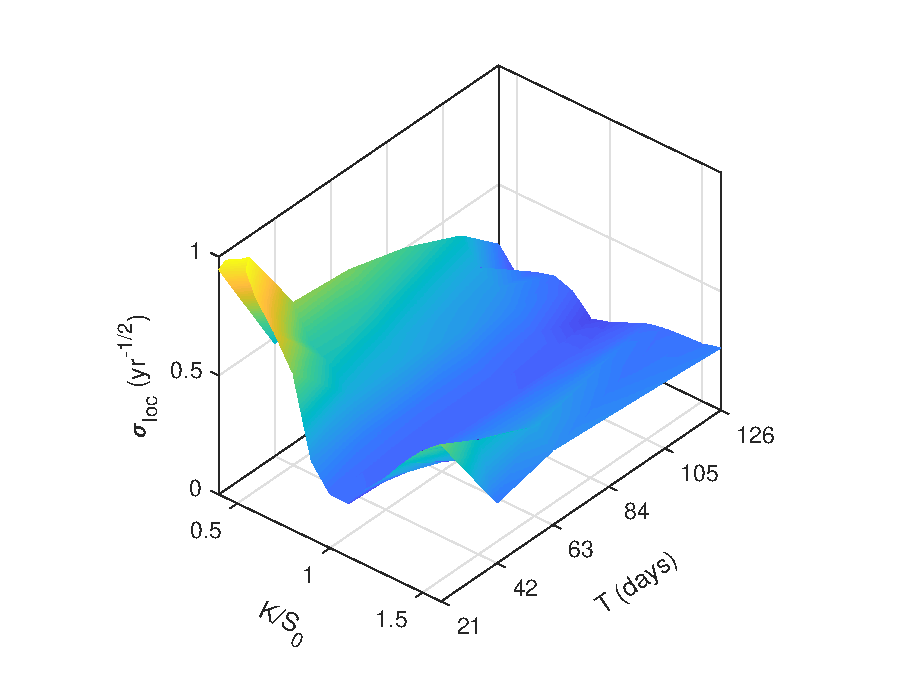
\includegraphics[width=0.49\linewidth,trim={1.7cm 0.45cm 2.cm 0.85cm},clip]{LocalV.eps}}
    \subfigure[$\sigma_{loc}$ contour plot]{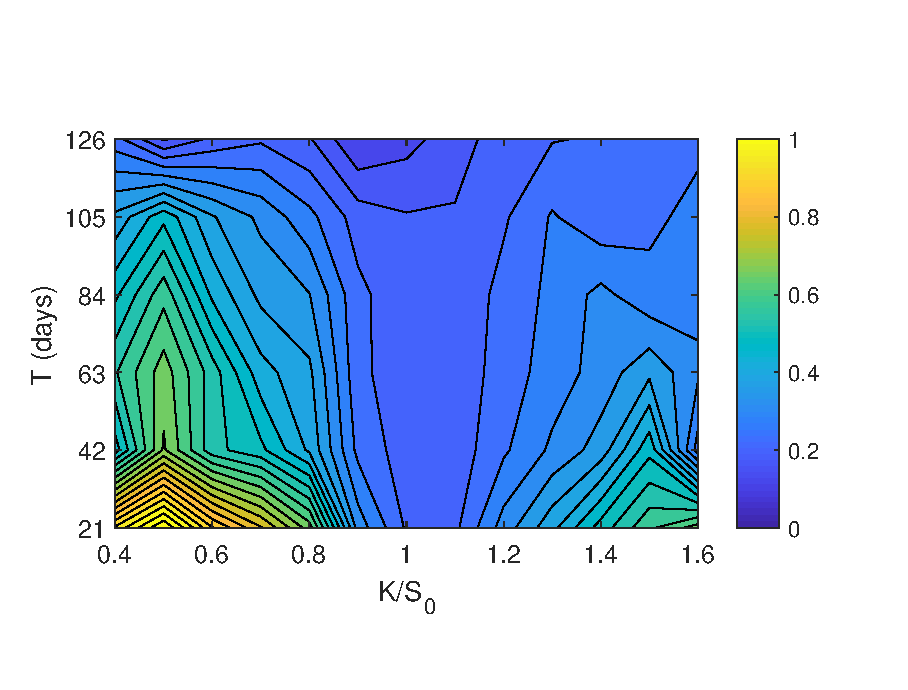
\includegraphics[width=0.49\linewidth,trim={0.2cm 0.5cm 1.25cm 1.55cm},clip]{LocalVC.eps}}
  \end{subfigmatrix}
    \caption[Local volatility surface and corresponding contour plot of the function obtained with Dupire's formula from the interpolated implied volatility surface.]{Local volatility surface (left) and corresponding contour plot (right) of the function obtained with Dupire's formula (eq.\eqref{dupire2}) from the interpolated implied volatility surface in \autoref{fig:DupImpV}.}\label{fig:DupLocVol}
\end{figure}   


Though we can't obtain any theoretical results, due to a lack of closed-form solutions in this model, we are able to simulate stock prices using the method described in \autoref{subsubsection:EulerMaruyama discretization} and with them obtain the option prices.
The results of these simulations are shown in \autoref{fig:Dup}, along with the confidence bands and the original market data. To prevent volatilities from becoming too high, we implemented a maximum cutoff value of $\sigma_{max}$=$1.5\SI{}{\year\tothe{-1/2}}$, limiting the volatilities sampled from the surface.

\vfill
\newpage

\begin{figure}[H]
  \begin{subfigmatrix}{2}
    \subfigure[$T=21$ days]{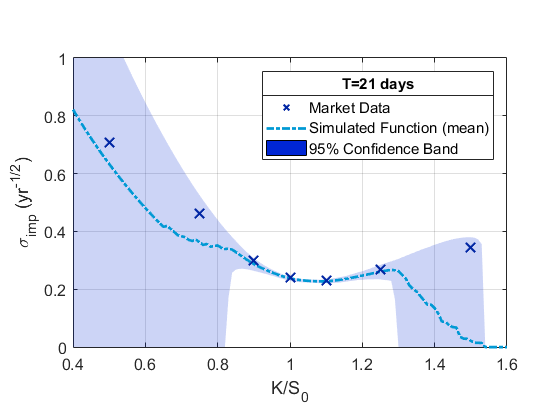
\includegraphics[width=0.49\linewidth,trim={0.25cm 0.45cm 1.1cm 1.4cm},clip]{Dup1.png}}
    \subfigure[$T=42$ days]{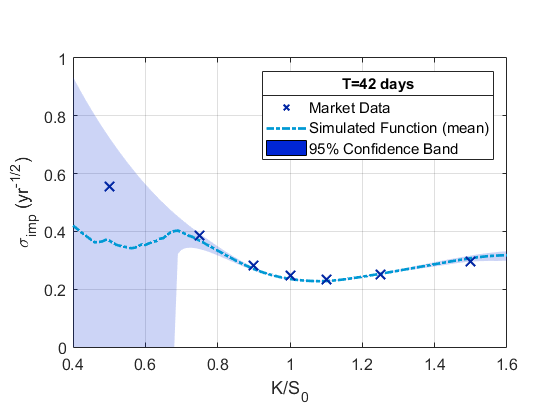
\includegraphics[width=0.49\linewidth,trim={0.25cm 0.45cm 1.1cm 1.4cm},clip]{Dup2.png}}
    \subfigure[$T=63$ days]{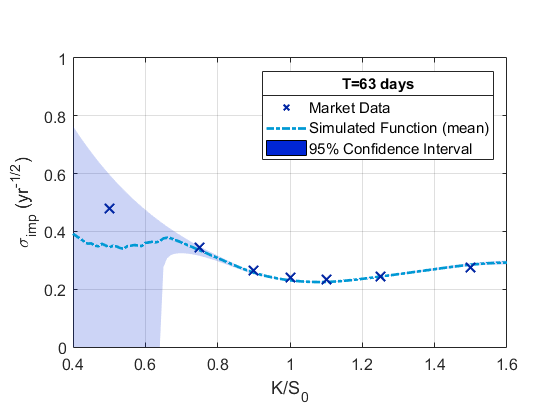
\includegraphics[width=0.49\linewidth,trim={0.25cm 0.45cm 1.1cm 1.4cm},clip]{Dup3.png}}
    \subfigure[$T=126$ days]{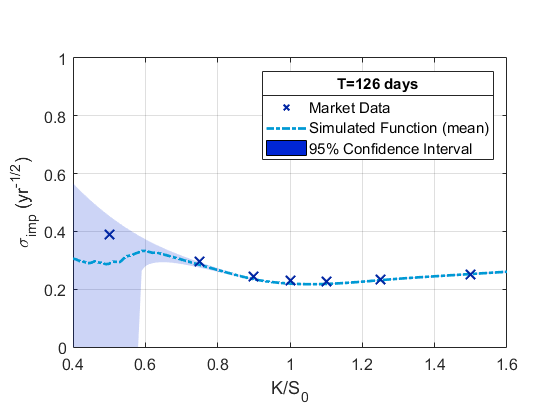
\includegraphics[width=0.49\linewidth,trim={0.25cm 0.45cm 1.1cm 1.4cm},clip]{Dup4.png}}
  \end{subfigmatrix}
  \caption[Implied volatility functions simulated with Monte Carlo under Dupire's local volatility model with their corresponding 95\% confidence band, plotted against the original market data.]{Implied volatility functions (light-blue dot-dashed) simulated with Monte Carlo under Dupire's local volatility model with their corresponding 95\% confidence band, plotted against the original market data (crosses).}
  \label{fig:Dup}
\end{figure}


As before, we now see the very large confidence bands for very low strikes. The cause of this behavior was identified on the constant volatility model (with independent fits). We can also observe the large confidence bands for high strikes in the earliest maturities, which has also already been discussed.

The great improvement of Dupire's model over the constant volatility model is the presence of the implied volatility smiles in the simulated implied volatilities. Furthermore, these smiles follow the market data almost perfectly for strikes near $S_0$.
We can therefore conclude that this model is clearly more adequate than the constant volatility model presented earlier, which is unsurprising.

The simulations shown in the plots of \autoref{fig:Dup} can be thought of as slices of a simulated implied volatility surface. Ideally, this surface would look exactly like the one shown in \autoref{fig:DupImpV}. However, in the regions where the simulations behave badly (large strikes for early maturities and low strikes), we expect there to be a very high amount of error in the simulations. This simulated surface is shown in \autoref{fig:DupS}, along with the simulated functions of the earlier plots and the market data. The respective contour plot is also represented.

\vfill
\newpage

\begin{figure}[H]
  \begin{subfigmatrix}{2}
    \subfigure[$\sigma_{imp}$ surface]{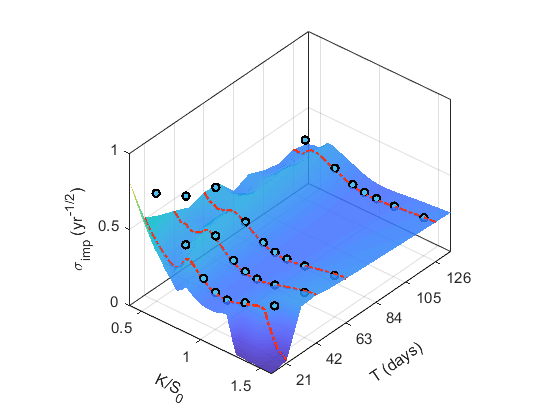
\includegraphics[width=0.49\linewidth,trim={1.7cm 0.45cm 1.9cm 0.85cm},clip]{DupS.png}}
    \subfigure[$\sigma_{imp}$ contour plot]{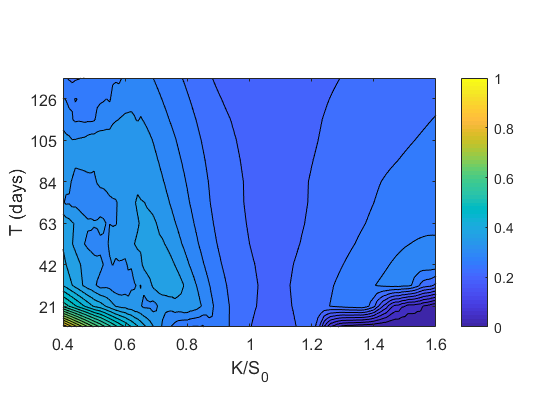
\includegraphics[width=0.49\linewidth,trim={0.2cm 0.5cm 1.25cm 1.55cm},clip]{DupSC.png}}
  \end{subfigmatrix}
    \caption[Implied volatility surface and corresponding contour plot simulated with Monte Carlo under Dupire's local volatility model plotted against the original market data and the simulated functions shown in \autoref{fig:Dup}.]{Implied volatility surface (left) and corresponding contour plot (right) simulated with Monte Carlo under Dupire's local volatility model plotted against the original market data (blue circles) and the simulated functions shown in \autoref{fig:Dup} (red dot-dashed lines).}\label{fig:DupS}
\end{figure}   


As expected, the amount of error is quite overwhelming in the regions where the Monte Carlo pricer performs badly. For the regions where the strike approaches $S_0$, the picture is quite different and the simulations closely follow the data, as expected.

For this model we do not show the table with the relative errors of the implied volatilities and prices, as we did for the constant volatility models, for the simple reason that previously we used the theoretical implied volatilities (i.e. red full lines in Figures \ref{fig:ConstVol} and \ref{fig:ConstVol2}) to calculate the relative errors and not the simulated curves (i.e. dot-dashed light blue lines in the same figures) and with Dupire's model there are no theoretical lines, only simulations. 


\vfill
\newpage

\section{Static SABR Model}
As we saw before, in the Static SABR model stock prices and volatilities are governed by the stochastic differential equations
\begin{subequations}
\begin{align}
&dS(t)=rS(t)dt+e^{-r(T-t)(1-\beta)}\sigma(t)(S(t))^\beta dW_1(t),\\
&d\sigma(t)=\nu\sigma(t) dW_2(t),
\end{align}
\end{subequations}
\noindent with $\alpha=\sigma(0)$ and where $W_1(t)$ and $W_2(t)$ have a constant correlation of $\rho$.

The closed-form solution, shown in eq.\eqref{sabr}, enables us to obtain the theoretical implied volatilities of options priced under this model and will be used in the calibration process.

Before calibrating the model to the market data, we should study the influence of each parameter of this model on the shape of the implied volatility curve, to better interpret the results. This influence is represented in \autoref{fig:SSparam}, where we plot the theoretical function while varying one parameter at a time, keeping all the others constant, thus directly observing that parameter's influence.


We should note that the influence of the parameters is more complicated than we show here. On the one hand, their impact depends on the maturity. However, for this effect to become evident, we would have to repeat all the plots in \autoref{fig:SSparam} for several maturities, which would simply become too cumbersome.
On the other hand, the parameters have combined effects on the curve shape. These influences would be quite difficult to represent. Furthermore, they are discussed in the original article by Hagan~\citep{Hagan}, and will, for these reasons, not be discussed here.
That being said, we can still have a general view of each parameter's impact on the curve.

\vfill
\newpage

\begin{figure}[H]
  \begin{subfigmatrix}{2}
    \subfigure[Dependence on $\alpha$]{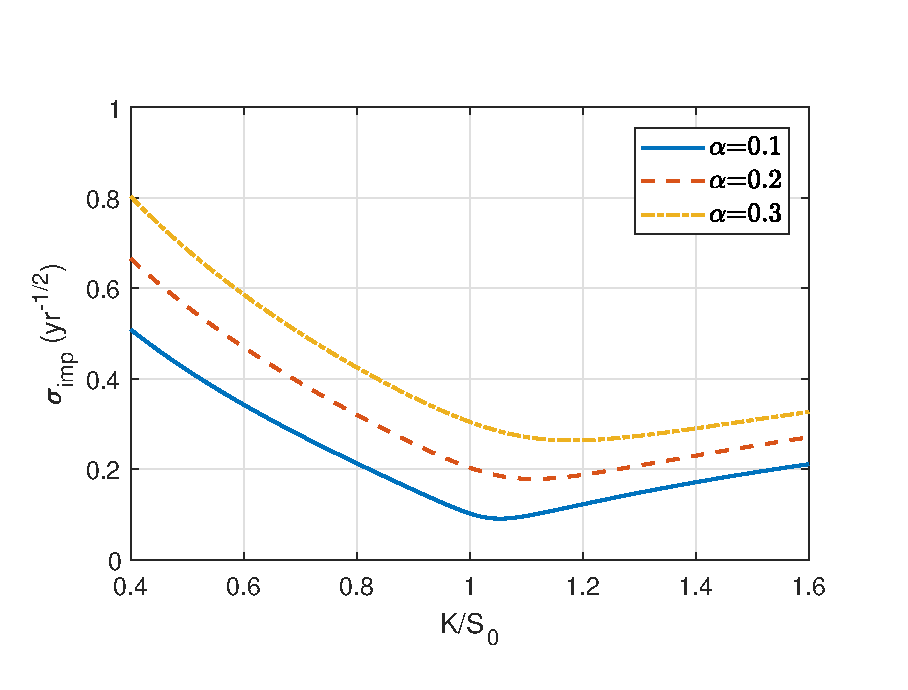
\includegraphics[width=0.49\linewidth,trim={0.25cm 0.45cm 1.1cm 1.4cm},clip]{SSalpha.eps}\label{SSa}}
    \subfigure[Dependence on $\beta$]{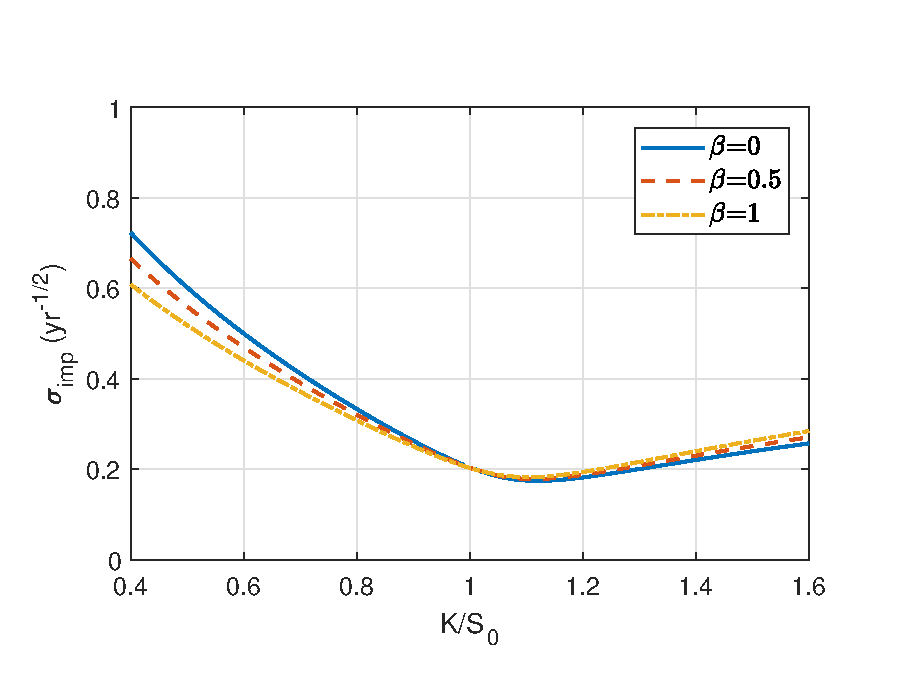
\includegraphics[width=0.49\linewidth,trim={0.25cm 0.45cm 1.1cm 1.4cm},clip]{SSbeta.eps}\label{SSb}}
    \subfigure[Dependence on $\rho$]{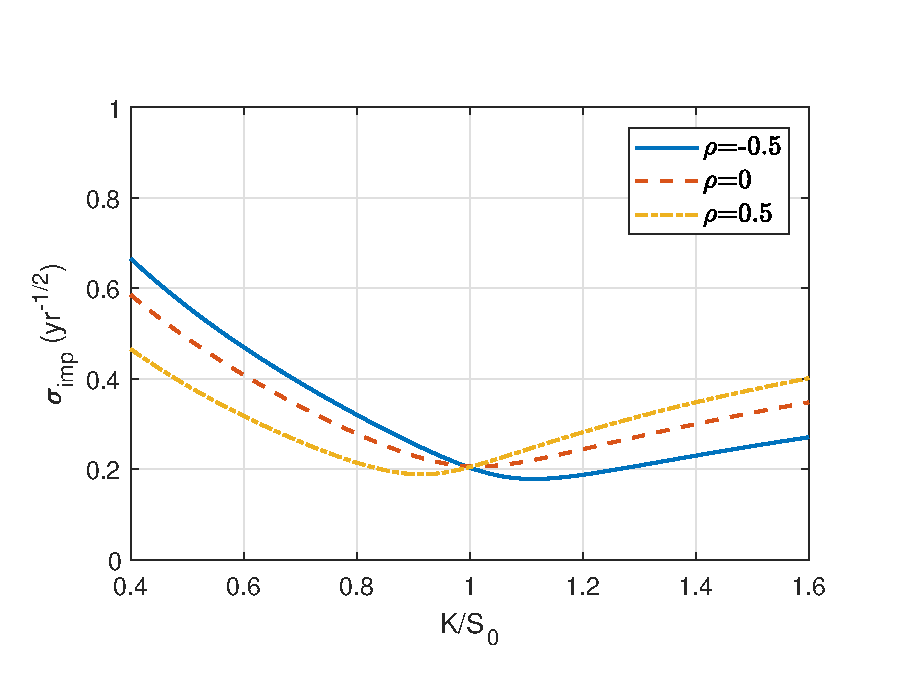
\includegraphics[width=0.49\linewidth,trim={0.25cm 0.45cm 1.1cm 1.4cm},clip]{SSrho.eps}\label{SSr}}
    \subfigure[Dependence on $\nu$]{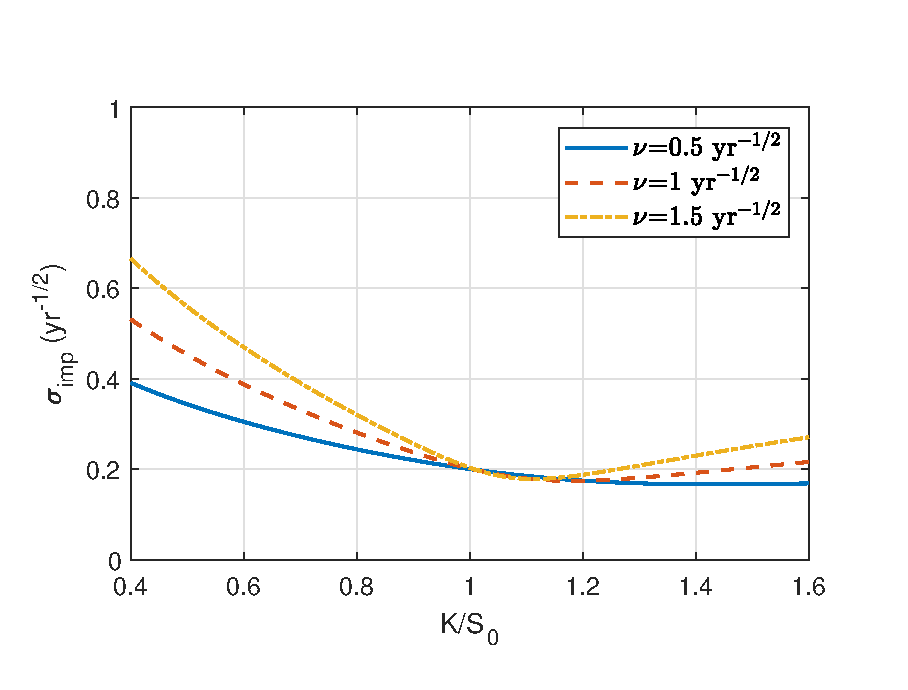
\includegraphics[width=0.49\linewidth,trim={0.25cm 0.45cm 1.1cm 1.4cm},clip]{SSnu.eps}\label{SSn}}
  \end{subfigmatrix}
  \caption[Dependence of the implied volatility curve on each of the Static SABR model parameters.]{Dependence of the implied volatility curve on each of the Static model SABR parameters. The default parameters used were $S_0=1\EUR$, $T=42$ days and $r=0$. Furthermore, on all plots, except when the dependence on a parameter is represented, the parameters used were $\alpha=0.2\SI{}{\year\tothe{-1/2}}$, $\beta=1$, $\rho=-0.5$ and $\nu=1.5\SI{}{\year\tothe{-1/2}}$.}
  \label{fig:SSparam}
\end{figure}

In Figure \autoref{SSa} we see that the parameter $\alpha$, which corresponds to the initial value of the volatility process, has quite an impact on the implied volatility curve. We can see that this parameter seems to control the height of the curve. This is indeed expected, because the implied volatility and the stochastic (local) volatility are inherently related. Increasing $\alpha$ is expected to shift the volatility process to higher values, thus increasing the resulting implied volatility.

The influence of the parameter $\beta$, which is an exponent in the stock price process, is represented in Figure \autoref{SSb}. The impact of this parameter seems to be almost negligible. Indeed, at a single point in time, the implied volatility curve barely depends on this value, but this parameter becomes very important when time passes and the stock prices change. Hagan \textit{et al.}~\citep{Hagan} show that $\beta$ controls how the curve shifts when the stock prices move: if the stock price increases, the implied volatility curve at that time should shift to the right; for $\beta=0$, the curve also shifts downwards, whereas for $\beta=1$ it doesn't, moving only horizontally.
Despite this, because in Static SABR we are only fitting data for a single maturity, this parameter should barely have any influence in the resulting implied volatility function, though it will become quite relevant in the Dynamic SABR model, where maturity is taken into account.

In Figure \autoref{SSr} is represented the effect of the parameter $\rho$, the correlation between the stock price and the volatility processes.
We can see that this parameter impacts the skewness of the implied volatility curve. Because this parameter relates the stock price and volatility, in the case of a negative $\rho$ when the prices increase (decrease), the volatilities decrease (increase), so that options with higher (lower) strikes have lower (higher) associated volatilities. This justifies why we have a lower implied volatility for higher strikes and a higher implied volatility for lower strikes when the correlation is negative. The inverse logic can be applied for the positive $\rho$ curve observed.

Finally, the impact of the parameter $\nu$, the volatility of the volatility process, is shown in Figure \autoref{SSn}. This parameter seems to control the curvature of the implied volatility curve. It should be clear that higher values of $\nu$ result in greater changes in the volatility process, enabling, at times, the volatility to become quite large. This allows the stock price process to evolve quite erratically, thus making it easier for stock prices to reach higher values, making high strike options more valuable. This effect pushes their implied volatility upwards. The inverse effect also holds and a low $\nu$ will force the stochastic volatility process to become quite limited, preventing the stock prices from changing too much, and restraining them from reaching high strikes, pulling the implied volatility curve downwards.

\vfill
\newpage

We now present the results of the calibration as well as the simulations in \autoref{fig:SS}.



\begin{figure}[H]
  \begin{subfigmatrix}{2}
    \subfigure[$T=21$ days]{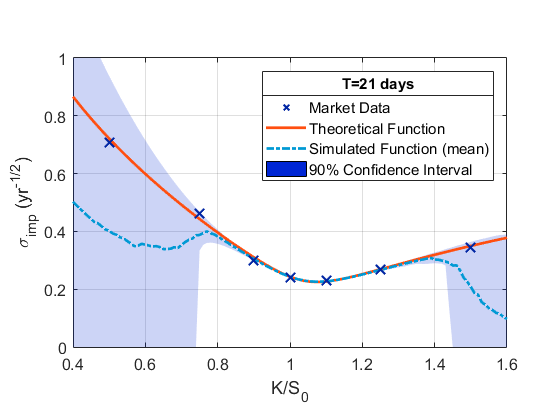
\includegraphics[width=0.49\linewidth,trim={0.25cm 0.45cm 1.1cm 1.4cm},clip]{SSABR1.png}}
    \subfigure[$T=42$ days]{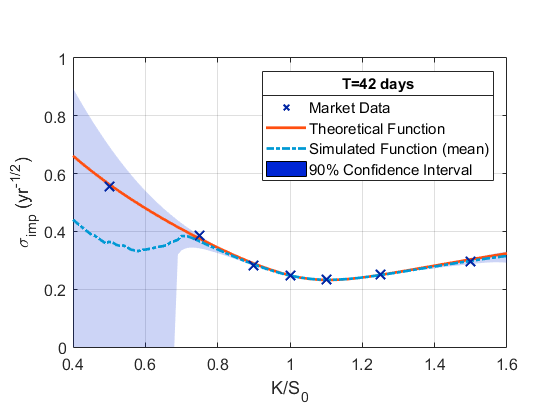
\includegraphics[width=0.49\linewidth,trim={0.25cm 0.45cm 1.1cm 1.4cm},clip]{SSABR2.png}}
    \subfigure[$T=63$ days]{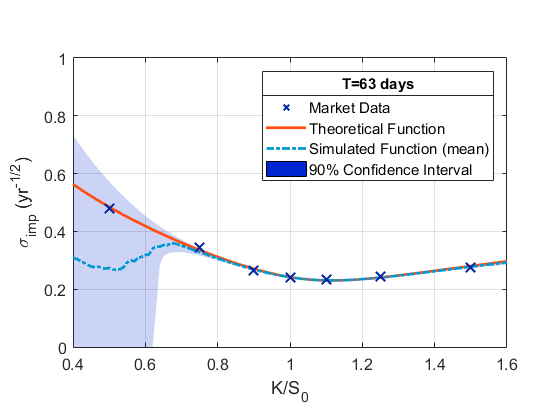
\includegraphics[width=0.49\linewidth,trim={0.25cm 0.45cm 1.1cm 1.4cm},clip]{SSABR3.png}}
    \subfigure[$T=126$ days]{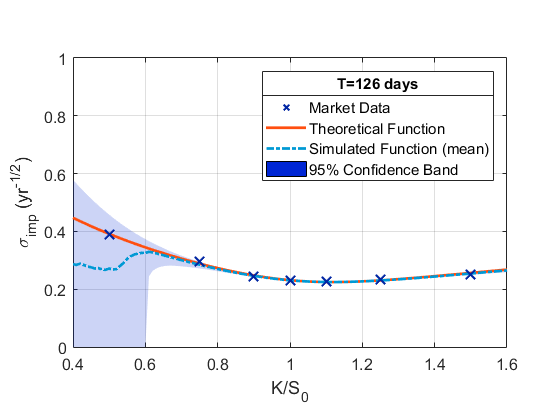
\includegraphics[width=0.49\linewidth,trim={0.25cm 0.45cm 1.1cm 1.4cm},clip]{SSABR4.png}}
  \end{subfigmatrix}
  \caption[Implied volatility functions fitted independently to the implied volatility data for different maturities under the static SABR model, plotted with their respective Monte Carlo simulated functions along with their 95\% confidence bands.]{Implied volatility functions (red lines) fitted independently to the implied volatility data (crosses) for different maturities under the static SABR model, plotted with their respective Monte Carlo simulated functions (light-blue dot-dashed lines) along with their 95\% confidence bands (blue region).}
  \label{fig:SS}
\end{figure}

As mentioned before, the Static SABR model is only expected to work for data on options with a single maturity. For this reason, we fitted the model to each maturity independently.
The parameters obtained in the calibration for each maturity are shown in \autoref{tab:SSR}.

\begin{table}[H]
    \centering
        \renewcommand{\arraystretch}{0.8}
\begin{tabular}{@{}lccccr@{}}
\toprule
 $T$(days) & $\alpha$ ($\SI{}{\year\tothe{-1/2}}$) & $\beta$ & $\rho$ & $\nu$ ($\SI{}{\year\tothe{-1/2}}$) & Cost \\ \midrule
21 & 0.2381 & 0.3766 & -0.3760 & 2.1022 & 0.0004 \\
42 & 0.2434 & 0.7362 & -0.3664 & 1.4451 & 0.0002\\
63 & 0.2375 & 0.7750 & -0.3119 & 1.1420 & 0.0001\\
126& 0.2267 & 0.8771 & -0.2383 & 0.8215 & 0.0001\\
\bottomrule
\end{tabular}
  \caption[Fitted parameters for each maturity (fitted independently) under static SABR model.]{Fitted parameters for each maturity (fitted independently) under static SABR model.}
  \label{tab:SSR}
\end{table}


We now analyze the results of this model. Observing the plots in \autoref{fig:SS} we see that the theoretical function (full red line), obtained by the closed form solution of the Static SABR model, fits the data extremely well through the whole range of strikes and for each of the maturities, which is further corroborated by the extremely low cost values in \autoref{tab:SSR}.

Though the model seems to fit almost perfectly to the data, the fits may not be very robust. The reason for this is the fact that we have an extremely small amount of data points (7 for each maturity) for the comparatively large number of parameters used (4 parameters in total). This will cause our model to overfit the data - for such a low amount of data (compared to the high number of parameters) we can find many possible combinations of parameters that fit the data just as well as the parameters found by the optimizer.


As for the simulated functions, we note that they very closely  the theoretical curves in the regions around $S_0$, indicating that the Monte Carlo pricer implementation was done correctly. This feature doesn't hold at the high strike region in the first maturity and the low strike regions of all maturities for the same reasons described earlier.

Examining now the calibrated parameters in \autoref{tab:SSR} we first note that the parameter $\alpha$ doesn't seem to vary too much between maturities, which is expected, since it controls the height of the implied volatility curve which doesn't seem to change too much in the plots. Furthermore, we see that these values are close to what is usually observed in the market.


The parameter $\beta$ appears to change wildly between maturities, though this is unsurprising since, as we saw, this parameter doesn't significantly affect the shape of the implied volatility function, meaning that different values of $\beta$ would fit the data equally well (i.e. overfitting).

As for the parameter $\rho$, we first note that it is always negative, which is expected from reality. It also seems to decrease with time which is expected for options with stock indices as underlying assets, as we mentioned in \autoref{subsection:Dynamic SABR Model}.

Finally, the parameter $\nu$ also seems to decrease with time. This should come as no surprise, since the curvature of the implied volatility function is expected to decrease with time, with the function becoming increasingly horizontal, as can be seen from the provided data and as we mentioned in \autoref{subsection:Dynamic SABR Model}. We should also note that the calibrated $\nu$ is quite large, which means that the volatility process evolves quite erratically.



\vfill
\newpage

The data of the fitted implied volatility and its respective option prices, along with their relative errors, can be found in \autoref{tab:SS}.
\begin{table}[H]
\centering
\renewcommand{\arraystretch}{0.8}
\begin{tabular}{@{}cccrcr@{}}
\toprule
$T$(days) & $K/S_0$ & $\sigma_{imp,\mathrm{mdl}}$($\SI{}{\year\tothe{-1/2}}$) & $\mathrm{Error}_{\sigma}(\%)$ & $C_{\mathrm{mdl}}$($\EUR$) & $\mathrm{Error}_{C}(\%)$ \\ \midrule
\multirow{7}{*}{21} & 0.50 & 0.7209 & 2 & \num{5.000E-01} & 0 \\
 & 0.75 & 0.4428 & 4 & \num{2.505E-01} & 0 \\
 & 0.90 & 0.3105 & 4 & \num{1.050E-01} & 1 \\
 & 1.00 & 0.2435 & 0 & \num{2.804E-02} & 0 \\
 & 1.10 & 0.2269 & 2 & \num{2.227E-03} & 8 \\
 & 1.25 & 0.2692 & 0 & \num{5.183E-05} & 3 \\
 & 1.50 & 0.3500 & 2 & \num{8.317E-07} & 45 \\ \midrule
\multirow{7}{*}{42} & 0.50 & 0.5631 & 1 & \num{5.001E-01} & 0 \\
 & 0.75 & 0.3751 & 3 & \num{2.515E-01} & 0 \\
 & 0.90 & 0.2891 & 2 & \num{1.114E-01} & 1 \\
 & 1.00 & 0.2481 & 1 & \num{4.039E-02} & 1 \\
 & 1.10 & 0.2322 & 1 & \num{8.194E-03} & 4 \\
 & 1.25 & 0.2497 & 1 & \num{5.746E-04} & 7 \\
 & 1.50 & 0.3033 & 2 & \num{2.120E-05} & 34 \\ \midrule
\multirow{7}{*}{63} & 0.50 & 0.4845 & 1 & \num{5.001E-01} & 0 \\
 & 0.75 & 0.3357 & 3 & \num{2.526E-01} & 0 \\
 & 0.90 & 0.2710 & 2 & \num{1.160E-01} & 1 \\
 & 1.00 & 0.2421 & 1 & \num{4.826E-02} & 1 \\
 & 1.10 & 0.2305 & 1 & \num{1.384E-02} & 3 \\
 & 1.25 & 0.2409 & 1 & \num{1.678E-03} & 7 \\
 & 1.50 & 0.2804 & 2 & \num{9.557E-05} & 25 \\ \midrule
\multirow{7}{*}{126} & 0.50 & 0.3914 & 1 & \num{5.004E-01} & 0 \\
 & 0.75 & 0.2887 & 2 & \num{2.563E-01} & 0 \\
 & 0.90 & 0.2479 & 1 & \num{1.279E-01} & 1 \\
 & 1.00 & 0.2314 & 1 & \num{6.522E-02} & 1 \\
 & 1.10 & 0.2251 & 1 & \num{2.817E-02} & 2 \\
 & 1.25 & 0.2309 & 1 & \num{7.177E-03} & 5 \\
 & 1.50 & 0.2567 & 2 & \num{9.822E-04} & 14 \\ \bottomrule
\end{tabular}
  \caption[Fitted implied volatilities and respective option prices along with their corresponding relative errors w.r.t. the provided data under the static SABR model.]{Fitted implied volatilities and respective option prices along with their corresponding relative errors w.r.t. the provided data under the static SABR model.}
  \label{tab:SS}
\end{table}

The phenomenon of high relative errors of the stock price for options with high strikes can be observed here as well, and will not be discussed again.

Furthermore, we can see that the errors in the implied volatilities are, at most, only $4\%$, which is extremely low, which further corroborates the low cost values shown in \autoref{tab:SSR}.

\vfill
\newpage

\section{Heston Model}
The Heston model is defined as
\begin{subequations}
\begin{align}
&dS(t)=rS(t)dt+\sqrt{\nu(t)}S(t)dW_1(t),\\
&d\nu(t)=\kappa(\overline{\nu}-\nu(t))dt+\eta\sqrt{\nu(t)}dW_2(t),
\end{align}
\end{subequations}
\noindent where $\nu_0=\nu(0)$ and with $W_1(t)$ and $W_2(t)$ having a constant correlation of $\rho$.

With the closed form solution of the Heston model, shown in eq.\eqref{CH}, we are able to find the theoretical prices of options priced under this model, which we can easily convert to implied volatilities. These last will be used in the calibration process.

As we did for the Static SABR model, we first study the influence of each parameter of the Heston model on the shape of the implied volatility curve, represented in \autoref{fig:Hparam}.

\vfill
\newpage

\begin{figure}[H]
  \begin{subfigmatrix}{2}
    \subfigure[Dependence on $\kappa$]{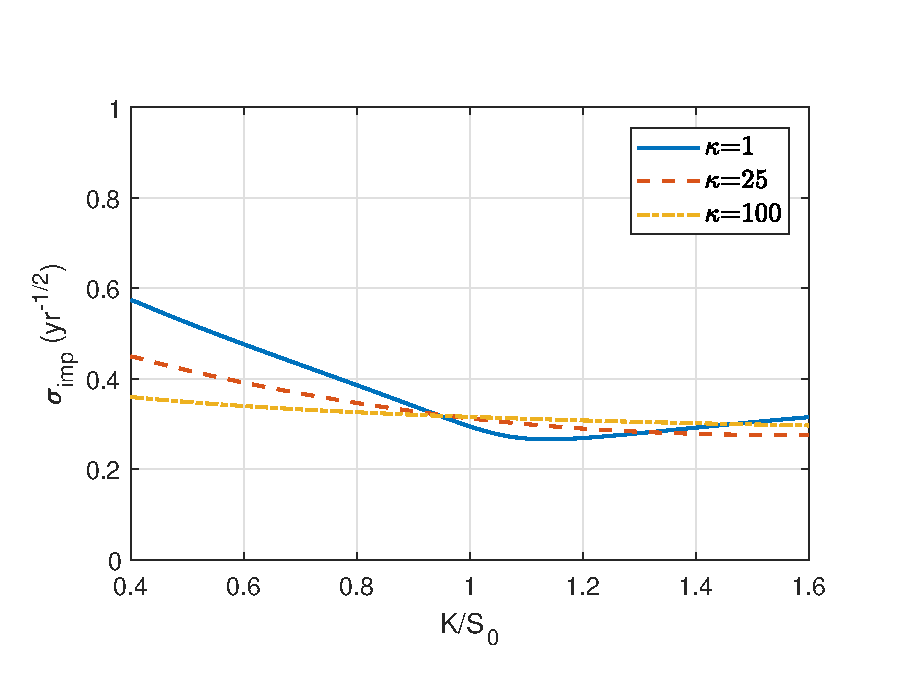
\includegraphics[width=0.49\linewidth,trim={0.25cm 0.45cm 1.1cm 1.4cm},clip]{Hkappa.eps}\label{Hk}}
    \subfigure[Dependence on $\overline{\nu}$]{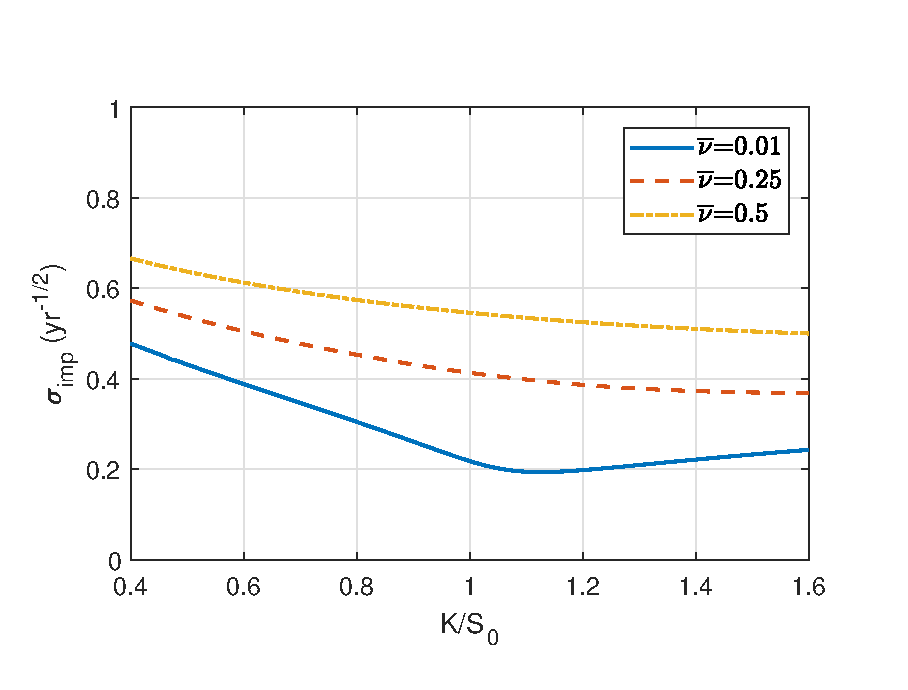
\includegraphics[width=0.49\linewidth,trim={0.25cm 0.45cm 1.1cm 1.4cm},clip]{Hnubar.eps}\label{Hnb}}
    \subfigure[Dependence on $\nu_0$]{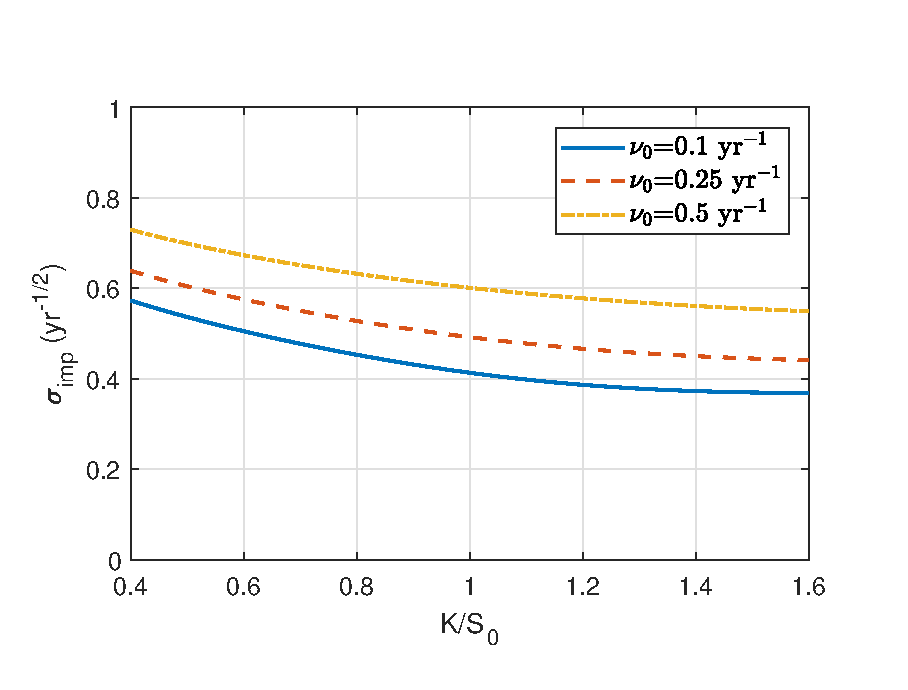
\includegraphics[width=0.49\linewidth,trim={0.25cm 0.45cm 1.1cm 1.4cm},clip]{Hnu0.eps}\label{Hn0}}
    \subfigure[Dependence on $\eta$]{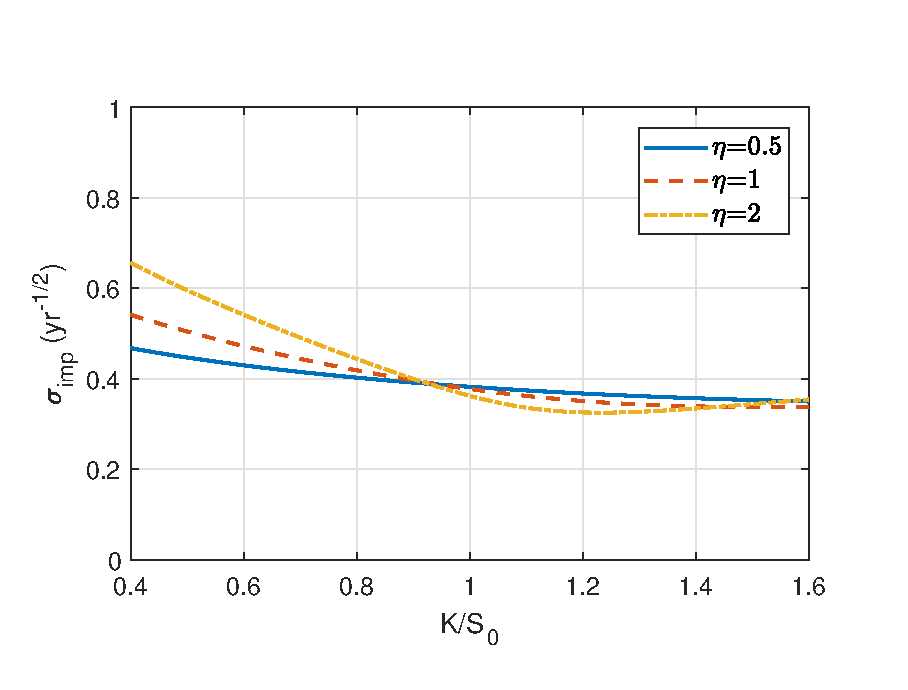
\includegraphics[width=0.49\linewidth,trim={0.25cm 0.45cm 1.1cm 1.4cm},clip]{Heta.eps}\label{He}}
        \subfigure[Dependence on $\rho$]{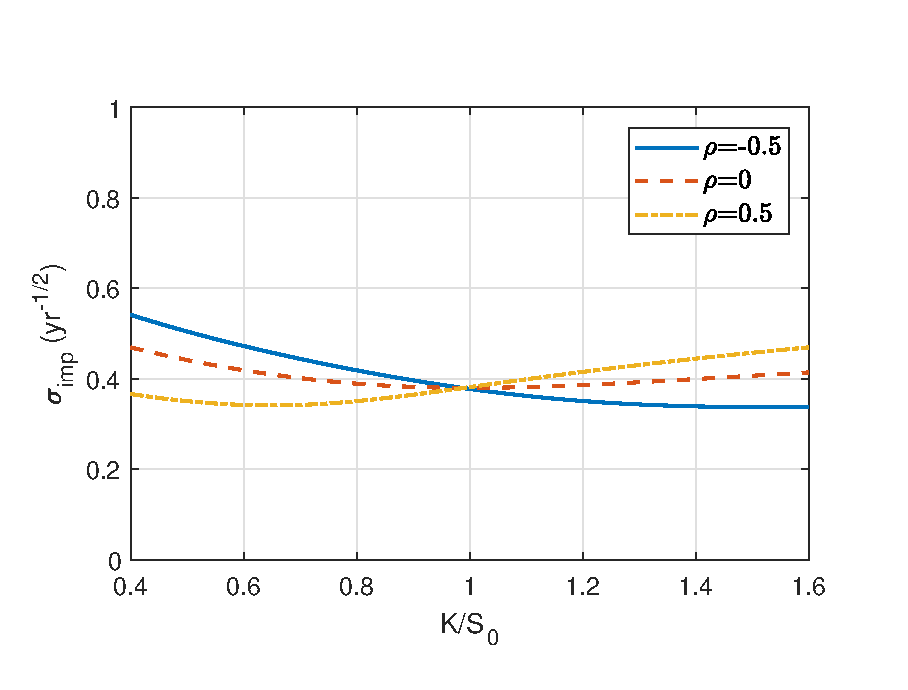
\includegraphics[width=0.49\linewidth,trim={0.25cm 0.45cm 1.1cm 1.4cm},clip]{Hrho.eps}\label{Hr}}
  \end{subfigmatrix}
  \caption[Dependence of the implied volatility curve on each of the Heston model parameters.]{Dependence of the implied volatility curve on each of the Heston model parameters. The default parameters used were $S_0=1\EUR$, $T=42$ days and $r=0$. Furthermore, on all plots, except when the dependence on a parameter is represented, the parameters used were $\kappa=10\SI{}{\year\tothe{-1}}$, $\overline{\nu}=0.25\SI{}{\year\tothe{-1}}$, $\nu_0=0.04\SI{}{\year\tothe{-1}}$, $\eta=1\SI{}{\year\tothe{-1}}$ and $\rho=-0.5$.}
  \label{fig:Hparam}
\end{figure}

The parameters $\kappa$, $\overline{\nu}$ and $\nu_0$ are inherently related to one another and their influence can only be understood if all are considered at the same time. The parameter $\overline{\nu}$ is the mean value of the variance (\emph{not} the volatility! $\nu(t)=\sigma^2(t)$), $\nu_0$ denotes the initial variance, and $\kappa$ is the mean-reversion rate, which controls how fast the variance tends to its mean value.

If the parameter $\kappa$ is very large, we expect the variance process to converge very fast to its mean value, $\overline{\nu}$. This means that the variance process $\nu(t)$ is not able to change significantly, as it is always pulled strongly towards $\overline{\nu}$, remaining roughly constant around this value. For this reason, options priced with such parameters would have an almost constant \emph{volatility}, and their implied volatility curve would tend to a horizontal line valued at the square root of $\overline{\nu}$ (i.e. the mean volatility, $\sqrt{\overline{\nu}}=\overline{\sigma}$).

On the other hand, if $\kappa$ is very small, the parameter $\overline{\nu}$ will barely have any influence on the implied volatility curve, and the variance process is able to change almost without restrain. This means that the parameter $\nu_0$ will have a large impact on the behavior of the variance process. A large $\nu_0$ enables the variance process to reach higher values (because it starts at a higher value) so that the implied volatility of options priced with these parameters is higher. A small $\nu_0$ would have the opposite effect, decreasing the implied volatility.

If we now have a moderate value for $\kappa$, both parameters $\overline{\nu}$ and $\nu_0$ are expected to have some impact on the implied volatility curve.

By examining Figures \autoref{Hnb} and \autoref{Hn0}, with a moderate value for $\kappa$, we see that the implied volatility curves increase/decrease as we increase/decrease the parameters $\overline{\nu}$ and $\nu_0$, which is precisely what we expect.
If we now look at Figure \autoref{Hk}, we can confirm that a large value for $\kappa$ (orange dot-dashed line) will produce an almost constant implied volatility curve around the square root of $\overline{\nu}$ ($\sqrt{\overline{\nu}}=\sqrt{0.25}=0.5\SI{}{\year\tothe{-1/2}}$).
For small values of $\kappa$ (blue full line), the influence of the parameter $\nu_0$ becomes more apparent - notice that the curve is pulled downwards since $\nu_0$ is lower than $\overline{\nu}$ -, and we no longer see the horizontal implied volatility curve from before, which is also expected.

The parameters $\eta$ and $\rho$ in the Heston model control the volatility of the variance process and the correlation of this process with the stock price process, respectively. They are very much related to the parameters $\nu$ and $\rho$ of the Static SABR process, respectively, and their impact on the implied volatility curve is the same. For this reason, they will not be discussed again here.

\vfill
\newpage

In \autoref{fig:H} we now show the results of the calibration and the simulations under this model.



\begin{figure}[H]
  \begin{subfigmatrix}{2}
    \subfigure[$T=21$ days]{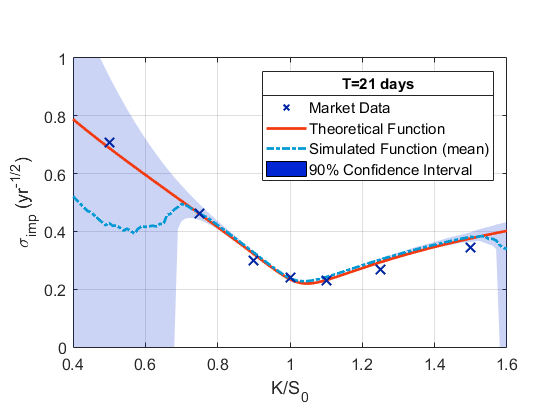
\includegraphics[width=0.49\linewidth,trim={0.25cm 0.45cm 1.1cm 1.4cm},clip]{H1.png}}
    \subfigure[$T=42$ days]{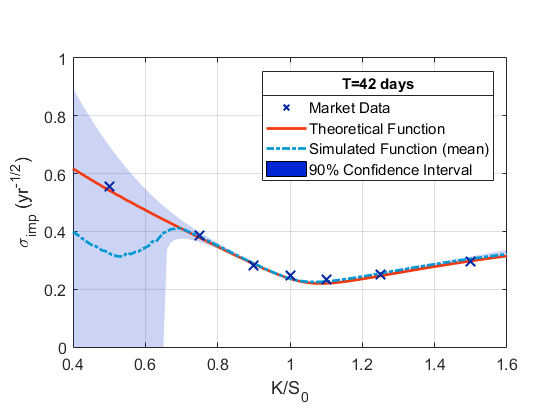
\includegraphics[width=0.49\linewidth,trim={0.25cm 0.45cm 1.1cm 1.4cm},clip]{H2.png}}
    \subfigure[$T=63$ days]{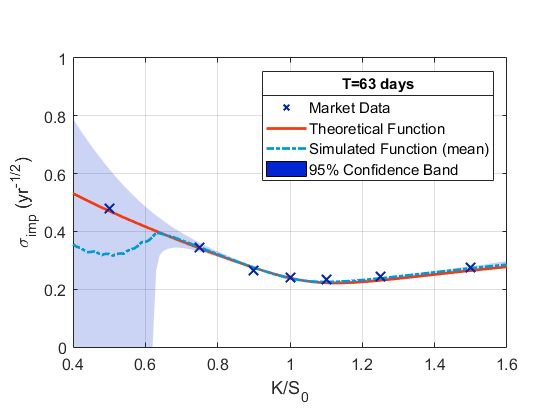
\includegraphics[width=0.49\linewidth,trim={0.25cm 0.45cm 1.1cm 1.4cm},clip]{H3.png}}
    \subfigure[$T=126$ days]{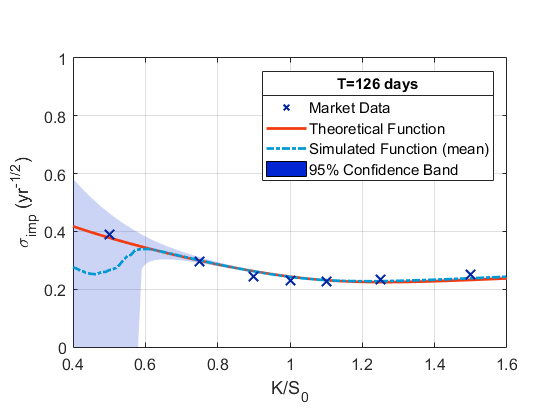
\includegraphics[width=0.49\linewidth,trim={0.25cm 0.45cm 1.1cm 1.4cm},clip]{H4.png}}
  \end{subfigmatrix}
  \caption[Implied volatility functions fitted simultaneously to the implied volatility data for different maturities under the Heston model, plotted with their respective Monte Carlo simulated functions along with their 95\% confidence bands.]{Implied volatility functions (red lines) fitted simultaneously to the implied volatility data (crosses) for different maturities under the Heston model, plotted with their respective Monte Carlo simulated functions (light-blue dot-dashed lines) along with their 95\% confidence bands (blue region).}
  \label{fig:H}
\end{figure}

The values of the calibrated parameters are shown in \autoref{tab:HR}.

\begin{table}[H]
    \centering
        \renewcommand{\arraystretch}{0.8}
\begin{tabular}{@{}lccccr@{}}
\toprule
$\kappa$ ($\SI{}{\year\tothe{-1}}$) & $\overline{\nu}$ ($\SI{}{\year\tothe{-1}}$) & $\nu_0$ ($\SI{}{\year\tothe{-1}}$) & $\rho$ & $\eta$ ($\SI{}{\year\tothe{-1}}$) & Cost \\ \midrule
53.4355 & 0.0653 & 0.1046 & -0.4086 & 6.2554 & 0.0025 \\
\bottomrule
\end{tabular}
  \caption[Fitted parameters for all maturities (fitted simultaneously) under the Heston model.]{Fitted parameters for all maturities (fitted simultaneously) under the Heston model.}
  \label{tab:HR}
\end{table}


Examining the plots in \autoref{fig:H} we see that the theoretical curves fit the data surprisingly well throughout all the maturities.
This is especially surprising when we note that the adjustment is made for the entire data set, with all the different maturities, unlike the Static SABR model, which was only fitted for single maturities, which means that the overfitting problem is attenuated.

Analyzing the fitted parameters' values, we begin by noting that $\kappa$ is quite large, which means that the variance process tends to its mean value $\overline{\nu}$ quite fast. It also means that the initial variance, $\nu_0$, has almost no influence on the shape of the fitted curves. We note furthermore that the mean variance, $\overline{\nu}$, corresponds to a mean volatility of $0.2555\SI{}{\year\tothe{-1/2}}$ ($\sqrt{\overline{\nu}}=\overline{\sigma}$), which is a typical value for volatilities observed in the market. The same applies to the initial variance, $\nu_0$. As for the correlation parameter, $\rho$, we note that it is negative, which is indeed expected from market behavior. Finally, the volatility of the variance process, $\eta$, is very large, which suggests that this process is very erratic.

Observing now the simulated curves and their respective confidence bands we again see that they fit the closed-form solutions extremely well in the region around $S_0$, indicating that the simulations agree with the predictions of the closed form solutions. The large confidence bands described before for the high strikes and early maturities and for the low strikes can also be found here. Because the phenomenon is the same as before, they will not be described again.



Both the simulated and theoretical implied volatility curves shown in the plots of \autoref{fig:H} for different maturities can be thought of as slices of implied volatility surfaces (one simulated, another theoretical). Similarly to what we did for the Dupire model, we again represent these surfaces and their respective contour plots in Figures \ref{fig:HS} and \ref{fig:HSSim}.


\begin{figure}[H]
  \begin{subfigmatrix}{2}
    \subfigure[$\sigma_{imp}$ surface]{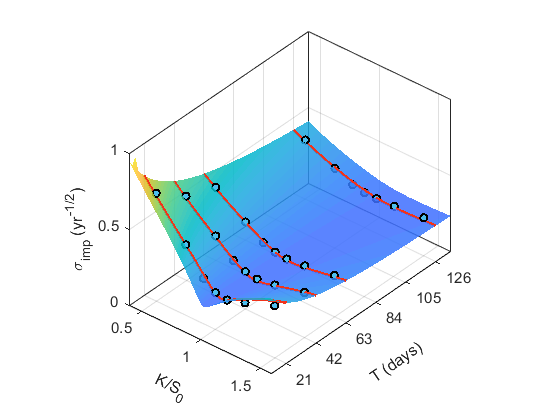
\includegraphics[width=0.49\linewidth,trim={1.7cm 0.45cm 2.35cm 0.85cm},clip]{HS.png}}
    \subfigure[$\sigma_{imp}$ contour plot]{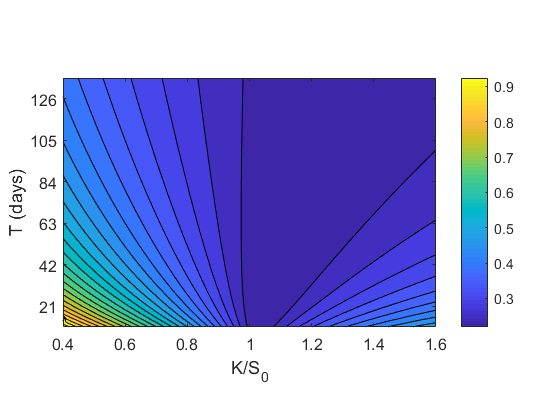
\includegraphics[width=0.49\linewidth,trim={0.2cm 0.5cm 1.25cm 1.55cm},clip]{HSC.png}}
  \end{subfigmatrix}
    \caption[Implied volatility surface and corresponding contour plot of the function fitted simultaneously to the implied volatility data for different maturities under the Heston model, plotted against the original market data and the fitted functions shown in \autoref{fig:H}.]{Implied volatility surface (left) and corresponding contour plot (right) of the function fitted simultaneously to the implied volatility data for different maturities under the Heston model, plotted against the original market data (blue circles) and the fitted functions shown in \autoref{fig:H} (red lines).}\label{fig:HS}
\end{figure}   

\vfill
\newpage

\begin{figure}[H]
  \begin{subfigmatrix}{2}
    \subfigure[$\sigma_{imp}$ surface]{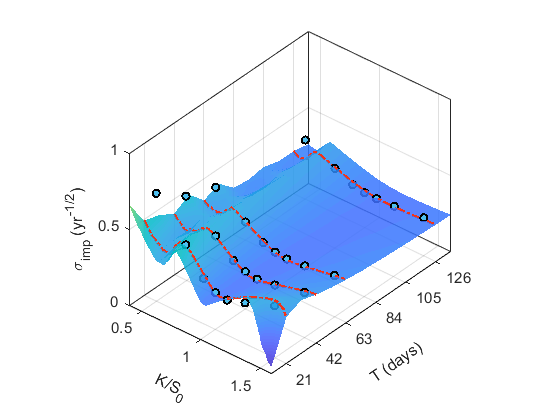
\includegraphics[width=0.49\linewidth,trim={1.7cm 0.45cm 2.35cm 0.85cm},clip]{HSSim.png}}
    \subfigure[$\sigma_{imp}$ contour plot]{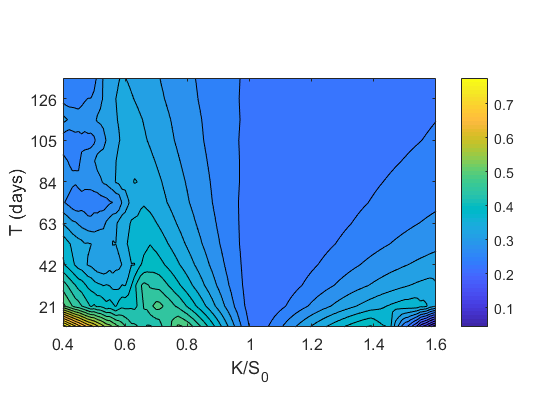
\includegraphics[width=0.49\linewidth,trim={0.2cm 0.5cm 1.25cm 1.55cm},clip]{HSCSim.png}}
  \end{subfigmatrix}
    \caption[Implied volatility surface and corresponding contour plot of the function simulated using the Monte Carlo method with the fitted parameters shown in \autoref{tab:HR}, under the Heston model, plotted against the original market data and the simulated functions shown in \autoref{fig:H}.]{Implied volatility surface (left) and corresponding contour plot (right) of the function simulated using the Monte Carlo method with the fitted parameters shown in \autoref{tab:HR}, under the Heston model, plotted against the original market data (blue circles) and the simulated functions shown in \autoref{fig:H} (red dot-dashed lines).}\label{fig:HSSim}
\end{figure} 


The surfaces and contour plots shown in Figures \ref{fig:HS} and \ref{fig:HSSim} should, ideally, replicate the surface and contour plot shown in \autoref{fig:DupImpV}, since these last correspond to the real (\emph{interpolated}) implied volatility surface. The simulated theoretical surface mimics the real function very well, which is expected, since the fits adjusted greatly to the data.
As for the simulated surface, we can see the expected noisy region for the low strikes. The simulations around $S_0$ are very close to the ideal values, though, as we can see from the comparison of the contour plots.

\vfill
\newpage

As before, we show in \autoref{tab:H} the implied volatilities and their respective option prices as well as their relative errors.

\begin{table}[H]
\centering
\renewcommand{\arraystretch}{0.8}
\begin{tabular}{@{}cccrcr@{}}
\toprule
$T$(days) & $K/S_0$ & $\sigma_{imp,\mathrm{mdl}}$($\SI{}{\year\tothe{-1/2}}$) & $\mathrm{Error}_{\sigma}(\%)$ & $C_{\mathrm{mdl}}$($\EUR$) & $\mathrm{Error}_{C}(\%)$ \\ \midrule
\multirow{7}{*}{21} & 0.50 & 0.6886 & 3 & \num{5.000E-01} & 0 \\
 & 0.75 & 0.4604 & 1 & \num{2.506E-01} & 0 \\
 & 0.90 & 0.3216 & 8 & \num{1.056E-01} & 1 \\
 & 1.00 & 0.2346 & 3 & \num{2.702E-02} & 3 \\
 & 1.10 & 0.2316 & 0 & \num{2.429E-03} & 0 \\
 & 1.25 & 0.2935 & 9 & \num{1.243E-04} & 133 \\
 & 1.50 & 0.3759 & 10 & \num{2.958E-06} & 415 \\ \midrule
\multirow{7}{*}{42} & 0.50 & 0.5422 & 2 & \num{5.000E-01} & 0 \\
 & 0.75 & 0.3781 & 2 & \num{2.516E-01} & 0 \\
 & 0.90 & 0.2873 & 2 & \num{1.112E-01} & 0 \\
 & 1.00 & 0.2366 & 4 & \num{3.852E-02} & 4 \\
 & 1.10 & 0.2205 & 6 & \num{7.021E-03} & 18 \\
 & 1.25 & 0.2463 & 2 & \num{5.203E-04} & 16 \\
 & 1.50 & 0.2979 & 0 & \num{1.661E-05} & 5 \\ \midrule
\multirow{7}{*}{63} & 0.50 & 0.4709 & 2 & \num{5.001E-01} & 0 \\
 & 0.75 & 0.3420 & 1 & \num{2.528E-01} & 0 \\
 & 0.90 & 0.2748 & 3 & \num{1.166E-01} & 1 \\
 & 1.00 & 0.2392 & 0 & \num{4.768E-02} & 0 \\
 & 1.10 & 0.2224 & 5 & \num{1.265E-02} & 11 \\
 & 1.25 & 0.2310 & 5 & \num{1.312E-03} & 27 \\
 & 1.50 & 0.2649 & 4 & \num{4.968E-05} & 35 \\ \midrule
\multirow{7}{*}{126} & 0.50 & 0.3784 & 2 & \num{5.003E-01} & 0 \\
 & 0.75 & 0.2993 & 1 & \num{2.573E-01} & 0 \\
 & 0.90 & 0.2626 & 7 & \num{1.312E-01} & 3 \\
 & 1.00 & 0.2439 & 6 & \num{6.870E-02} & 6 \\
 & 1.10 & 0.2314 & 2 & \num{2.973E-02} & 4 \\
 & 1.25 & 0.2248 & 4 & \num{6.453E-03} & 15 \\
 & 1.50 & 0.2324 & 8 & \num{4.446E-04} & 48 \\ \bottomrule
\end{tabular}
  \caption[Fitted implied volatilities and respective option prices along with their corresponding relative errors w.r.t. the provided data under the Heston model.]{Fitted implied volatilities and respective option prices along with their corresponding relative errors w.r.t. the provided data under the Heston model.}
  \label{tab:H}
\end{table}

We can see that the relative errors shown in \autoref{tab:H} for the Heston model are higher than those for the Static SABR model, in \autoref{tab:SS}. This is expected from the comparison of their respective costs and was discussed previously.
Not much else can be added that hasn't been observed and discussed before.




\vfill
\newpage


\section{Dynamic SABR Model}

We now consider the Dynamic SABR Model, for which the stock price and volatility processes were assumed to follow
\begin{subequations}
\begin{align}
&dS(t)=rS(t)dt+e^{-r(T-t)(1-\beta)}\sigma(t) (S(t))^\beta dW_1(t),\\
&d\sigma(t)=\nu(t)\sigma(t) dW_2(t),
\end{align}
\end{subequations}
\noindent with the volatility of the volatility process, $\nu(t)$, and the correlation between $W_1(t)$ and $W_2(t)$, $\rho(t)$, being two functions of time.

To model these functions, we chose
\begin{equation}
\rho(t)=\rho_0e^{-at},
\end{equation}
\begin{equation}
\nu(t)=\nu_0e^{-bt},
\end{equation}
\noindent with $\rho_0\in[-1,1]$, $\nu_0>0$, $a>0$ and $b>0$.


The parameters used in the Dynamic SABR model are similar to those used in the Static SABR model and an easy connection can be made between them. Their influence on the implied volatility curve will therefore be the same and, for this reason, they will not be represented again here.

We fitted the Dynamic SABR model to the implied volatility data for all maturities. The fitted theoretical curves (obtained with the closed-form solution in eq.\eqref{dynsabr}) and their simulated counterparts are shown in \autoref{fig:DS}.

\vfill
\newpage

\begin{figure}[H]
  \begin{subfigmatrix}{2}
    \subfigure[$T=21$ days]{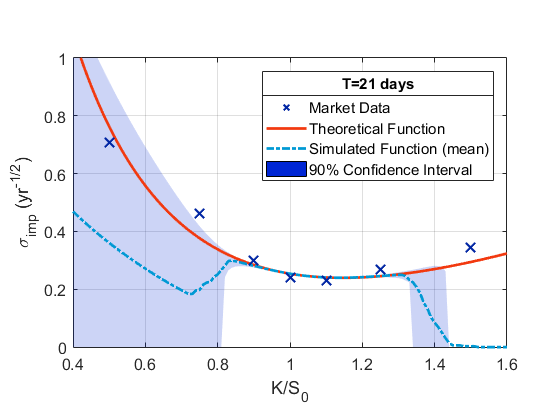
\includegraphics[width=0.49\linewidth,trim={0.25cm 0.45cm 1.1cm 1.4cm},clip]{DS1.png}}
    \subfigure[$T=42$ days]{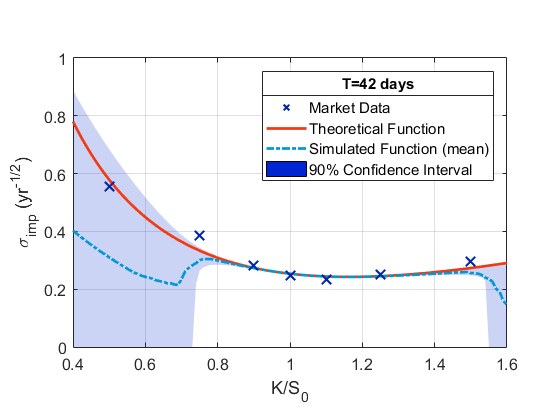
\includegraphics[width=0.49\linewidth,trim={0.25cm 0.45cm 1.1cm 1.4cm},clip]{DS2.png}}
    \subfigure[$T=63$ days]{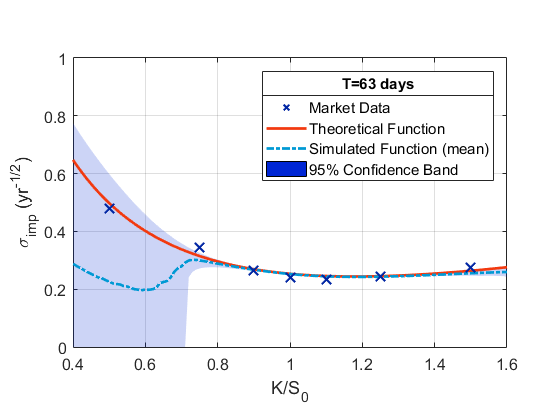
\includegraphics[width=0.49\linewidth,trim={0.25cm 0.45cm 1.1cm 1.4cm},clip]{DS3.png}}
    \subfigure[$T=126$ days]{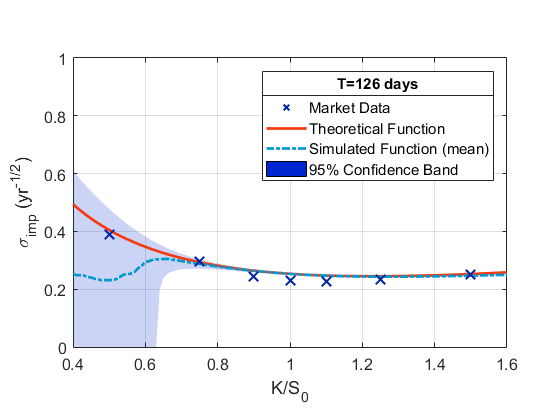
\includegraphics[width=0.49\linewidth,trim={0.25cm 0.45cm 1.1cm 1.4cm},clip]{DS4.png}}
  \end{subfigmatrix}
  \caption[Implied volatility functions fitted simultaneously to the implied volatility data for different maturities under the dynamic SABR model, plotted with their respective Monte Carlo simulated functions along with their 95\% confidence bands.]{Implied volatility functions (red lines) fitted simultaneously to the implied volatility data (crosses) for different maturities under the dynamic SABR model, plotted with their respective Monte Carlo simulated functions (light-blue dot-dashed lines) along with their 95\% confidence bands (blue region).}
  \label{fig:DS}
\end{figure}

The calibrated parameters obtained from the fit are shown in \autoref{tab:DSR}.

\begin{table}[H]
    \centering
        \renewcommand{\arraystretch}{0.8}
\begin{tabular}{@{}lcccccr@{}}
\toprule
$\alpha$ ($\SI{}{\year\tothe{-1/2}}$) & $\beta$ & $\rho_0$ & $a$ ($\SI{}{\year\tothe{-1}}$) & $\nu_0$ ($\SI{}{\year\tothe{-1/2}}$) & $b$ ($\SI{}{\year\tothe{-1}}$) & Cost \\ \midrule
0.2540 & 0.6348 & -0.4166 & 0 & 1.8673 & 41.6943 & 0.0108 \\
\bottomrule
\end{tabular}
  \caption[Fitted parameters for all maturities (fitted simultaneously) under the dynamic SABR model.]{Fitted parameters for all maturities (fitted simultaneously) under the dynamic SABR model.}
  \label{tab:DSR}
\end{table}


We now consider the adjustments above. Observing the theoretical curves in \autoref{fig:DS} we can see that they fit the market data relatively well, especially for the later maturities.

Analyzing the calibrated parameters in \autoref{tab:DSR}, we begin by noting that the value of $\alpha$ is typical from market observations. As we mentioned previously, the parameter $\beta$ controls how the implied volatility curve shifts when the stock prices move, and the calibrated value indicates that when the stock prices increase, the curve not only shifts to the right but also downwards, though only slightly.

The parameter $a$ being $0$ means that the correlation function, $\rho(t)$, is stuck at $\rho_0$ through time, and the parameter $b$ being very large means that the volatility of the volatility function, $\nu(t)$, goes to $0$ extremely fast (e.g. at the end of the first month, this parameter is only $\nu(t=1$ month$)=0.0578\SI{}{\year\tothe{-1}}$). These results are very inconsistent with what we observed in the Static SABR model, where both the correlations (in absolute value) and the volatilities of the volatility decreased (slowly) with time. This seems to suggest that the functions chosen to model these two parameters were not appropriate.


Considering now the simulated curves, we see that they accurately follow the theoretical curves for the regions around $S_0$, behaving badly only for the low strike regions and for high strikes with low maturities. This has been observed before in all models and is therefore expected.


As we did for the Heston model, we now present the theoretical and simulated implied volatility surfaces of which the plots in \autoref{fig:DS} are slices. 
These surfaces and their respective contour plots are shown in Figures \ref{fig:DSS} and \ref{fig:DSSSim}.

\vfill
\newpage

\begin{figure}[H]
  \begin{subfigmatrix}{2}
    \subfigure[$\sigma_{imp}$ surface]{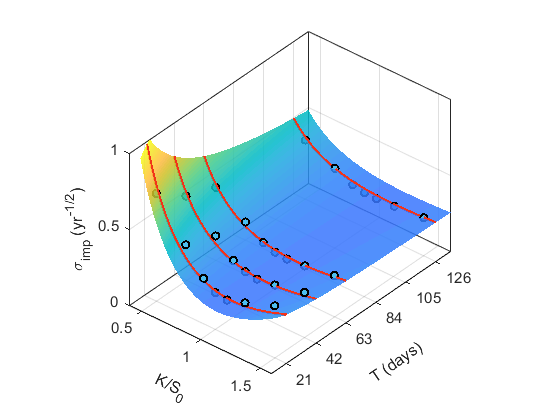
\includegraphics[width=0.49\linewidth,trim={1.7cm 0.45cm 2.35cm 0.85cm},clip]{DSS.png}}
    \subfigure[$\sigma_{imp}$ contour plot]{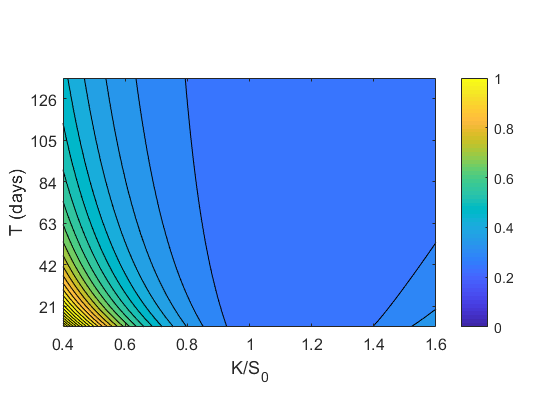
\includegraphics[width=0.49\linewidth,trim={0.2cm 0.5cm 1.25cm 1.55cm},clip]{DSSC.png}}
  \end{subfigmatrix}
    \caption[Implied volatility surface and corresponding contour plot of the function fitted simultaneously to the implied volatility data for different maturities under the dynamic SABR model, plotted against the original market data and the fitted functions shown in \autoref{fig:DS}.]{Implied volatility surface (left) and corresponding contour plot (right) of the function fitted simultaneously to the implied volatility data for different maturities under the dynamic SABR model, plotted against the original market data (blue circles) and the fitted functions shown in \autoref{fig:DS} (red lines).}\label{fig:DSS}
\end{figure}   


\begin{figure}[H]
  \begin{subfigmatrix}{2}
    \subfigure[$\sigma_{imp}$ surface]{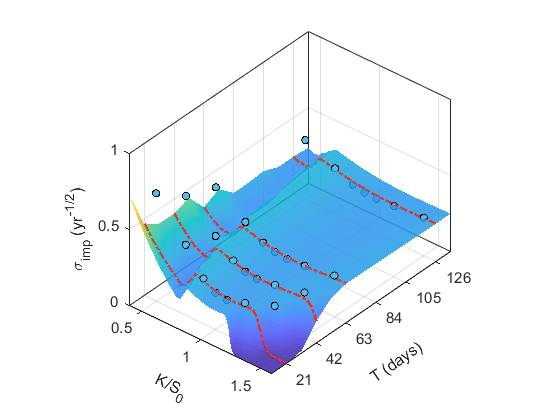
\includegraphics[width=0.49\linewidth,trim={1.7cm 0.45cm 2.35cm 0.85cm},clip]{DSSSim.png}}
    \subfigure[$\sigma_{imp}$ contour plot]{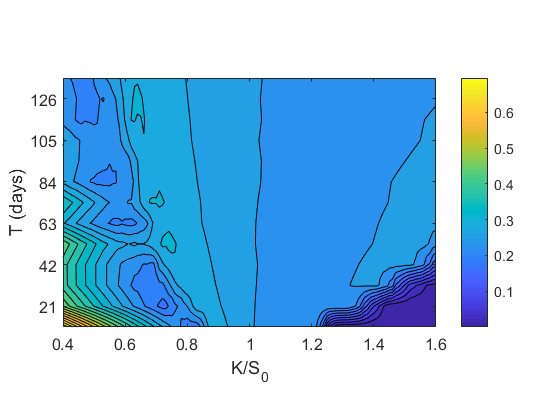
\includegraphics[width=0.49\linewidth,trim={0.2cm 0.5cm 1.25cm 1.55cm},clip]{DSSCSim.png}}
  \end{subfigmatrix}
    \caption[Implied volatility surface and corresponding contour plot of the function simulated using the Monte Carlo method with the fitted parameters shown in \autoref{tab:DSR}, under the dynamic SABR model, plotted against the original market data and the simulated functions shown in \autoref{fig:DS}.]{Implied volatility surface (left) and corresponding contour plot (right) of the function simulated using the Monte Carlo method with the fitted parameters shown in \autoref{tab:DSR}, under the dynamic SABR model, plotted against the original market data (blue circles) and the simulated functions shown in \autoref{fig:DS} (red dot-dashed lines).}\label{fig:DSSSim}
\end{figure} 


As stated before, ideally the plots in these two Figures would perfectly mimic the surface shown in \autoref{fig:DupImpV}. This obviously doesn't occur. The theoretical surface plot in \autoref{fig:DSS} seems to be flatter than the actual surface in the regions around $S_0$ (notice the wider contours in this region) whereas it increases quite abruptly for low strikes.
As for the simulated surface in \autoref{fig:DSSSim}, in the regions where the simulations are expected to behave badly, a large amount of error can be observed, as is expected.


Finally, we show in \autoref{tab:DS} the implied volatility and price data for the fits presented before, along with their respective relative errors.

\begin{table}[H]
\centering
\renewcommand{\arraystretch}{0.8}
\begin{tabular}{@{}cccrcr@{}}
\toprule
$T$(days) & $K/S_0$ & $\sigma_{imp,\mathrm{mdl}}$($\SI{}{\year\tothe{-1/2}}$) & $\mathrm{Error}_{\sigma}(\%)$ & $C_{\mathrm{mdl}}$($\EUR$) & $\mathrm{Error}_{C}(\%)$ \\ \midrule
\multirow{7}{*}{21} & 0.50 & 0.7625 & 8 & \num{5.000E-01} & 0 \\
 & 0.75 & 0.3765 & 19 & \num{2.501E-01} & 0 \\
 & 0.90 & 0.2843 & 5 & \num{1.037E-01} & 1 \\
 & 1.00 & 0.2540 & 5 & \num{2.924E-02} & 5 \\
 & 1.10 & 0.2410 & 4 & \num{2.858E-03} & 18 \\
 & 1.25 & 0.2454 & 9 & \num{1.760E-05} & 67 \\
 & 1.50 & 0.2944 & 14 & \num{1.857E-08} & 97 \\ \midrule
\multirow{7}{*}{42} & 0.50 & 0.5788 & 4 & \num{5.001E-01} & 0 \\
 & 0.75 & 0.3337 & 14 & \num{2.507E-01} & 0 \\
 & 0.90 & 0.2740 & 3 & \num{1.099E-01} & 1 \\
 & 1.00 & 0.2538 & 3 & \num{4.131E-02} & 3 \\
 & 1.10 & 0.2445 & 4 & \num{9.490E-03} & 11 \\
 & 1.25 & 0.2455 & 3 & \num{5.072E-04} & 18 \\
 & 1.50 & 0.2736 & 8 & \num{4.721E-06} & 70 \\ \midrule
\multirow{7}{*}{63} & 0.50 & 0.4980 & 4 & \num{5.001E-01} & 0 \\
 & 0.75 & 0.3150 & 9 & \num{2.518E-01} & 0 \\
 & 0.90 & 0.2695 & 1 & \num{1.158E-01} & 0 \\
 & 1.00 & 0.2537 & 6 & \num{5.057E-02} & 6 \\
 & 1.10 & 0.2460 & 6 & \num{1.619E-02} & 14 \\
 & 1.25 & 0.2455 & 1 & \num{1.868E-03} & 4 \\
 & 1.50 & 0.2642 & 4 & \num{4.810E-05} & 37 \\ \midrule
\multirow{7}{*}{126} & 0.50 & 0.4050 & 4 & \num{5.005E-01} & 0 \\
 & 0.75 & 0.2935 & 1 & \num{2.568E-01} & 0 \\
 & 0.90 & 0.2645 & 8 & \num{1.317E-01} & 4 \\
 & 1.00 & 0.2537 & 11 & \num{7.147E-02} & 11 \\
 & 1.10 & 0.2477 & 9 & \num{3.382E-02} & 18 \\
 & 1.25 & 0.2452 & 5 & \num{9.051E-03} & 20 \\
 & 1.50 & 0.2528 & 0 & \num{8.775E-04} & 2 \\ \bottomrule
\end{tabular}
  \caption[Fitted implied volatilities and respective option prices along with their corresponding relative errors w.r.t. the provided data under the dynamic SABR model.]{Fitted implied volatilities and respective option prices along with their corresponding relative errors w.r.t. the provided data under the dynamic SABR model.}
  \label{tab:DS}
\end{table}

By analyzing these results, we see that the relative errors increase when compared either with the Heston model or the Static SABR model, which is expected and has already been discussed.
Not much else can be added to the analysis of the results.


\vfill
\newpage

\section{Model Overview}
To round up all the results shown before and to facilitate comparisons between the models, in \autoref{tab:CostsCompare} we combine all the costs obtained from the training of all models. For the models where the training was done on each maturity independently (Constant Volatility with independent fits and Static SABR), the values shown denote the sum of the costs for all maturities, $\Sigma_{\mathrm{Costs}}$.
\begin{table}[H]
    \centering
        \renewcommand{\arraystretch}{0.8}
\begin{tabular}{@{}lcr@{}}
\toprule
 Model & Cost & $\Sigma_{\mathrm{Costs}}$ \\ \midrule
Constant Vol. (indep.) & - & 0.1150 \\
Constant Vol. (dep.) & 0.1248 & - \\
Dupire & - & - \\
Static SABR & - & 0.0008 \\
Heston & 0.0025 & - \\
Dynamic SABR & 0.0108\\
\bottomrule
\end{tabular}
  \caption[Comparison between the costs from all trained models.]{Comparison between the costs from all trained models.}
  \label{tab:CostsCompare}
\end{table}

We begin by noting that under the Constant Volatility model, the cost from the dependent fits is larger than the sum of the costs of the independent fits, which is unsurprising given that when fitting all maturities at once, the optimizer will find the implied volatility that minimizes the cost for all maturities, which will not necessarily be the one that minimizes the cost of each single maturity independently.

Regarding Dupire's model, as we stated before no closed form solution exists for this model, meaning that we aren't able to calculate the cost function. However, we saw before that the simulations from the Monte Carlo pricer presented the implied volatility smile phenomenon, suggesting that this model is more adequate that the constant volatility.

As for the Static SABR model, it showed a very significant improvement of $99.3\%$ over the cost of the constant volatility model with independent fits. This is no surprise, since the constant volatility model was expected to fit the data very badly and Static SABR fit it almost perfectly. These costs should be considered carefully, though, due to the overfitting mentioned earlier.


Regarding now the Heston and Dynamic SABR models, we can see that they also present a considerable improvement of $98.0\%$ and $91.3\%$, respectively, over the constant volatility model with dependent fits, which is also unsurprising for the same reasons as before.

Comparing now the cost resulting from the Heston model with that from Dynamic SABR, we see that even though both models fit the same data on a range of different maturities, Heston outperforms the Dynamic SABR quite significantly. This is further corroborated by the comparison of the theoretical functions in Figures \ref{fig:H} and \ref{fig:DS}, from which it is clear that the Heston model's curves seemed to better fit the data.



Finally, we can compare the sum of the costs from Static SABR with the costs from both Heston and Dynamic SABR models. To this regard we can say that the fact that we have a significantly lower cost for Static SABR model is unsurprising since the calibration performed under this model was done for multiple maturities, independently, meaning that a better fit is possible, at the cost of the aforementioned overfitting.

\vfill
\newpage

\section{Barrier Options}

Having trained all the models, we are now able to use our results on a slightly modified Monte Carlo method to price Barrier options. This has been described before in \autoref{subsection:Pricing options from simulations} along with all the expected shortcomings.

We priced several Barrier options with different barrier levels, using all the different models described before. In these simulations we used a single maturity of 42 days and the calibrated parameters for each of the models, shown earlier in their respective tables. The results of these simulations are shown in \autoref{fig:Barrier}.
For comparison, we also simulated some European option contracts, also represented in \autoref{fig:Barrier}.


\iffalse
From the Barrier option prices we extracted the corresponding implied volatilities, using eqs.\eqref{impvolform} and \eqref{barr2}, to compare the implied volatility curves with those shown in the previous sections.
We should also note that these curves are simulated (mean of multiple Monte Carlo simulations) and not theoretical, as there are no closed-form solutions for the prices of Barrier options under each of the used models.
\fi


\vfill
\newpage

\begin{figure}[H]
  \begin{subfigmatrix}{2}
    \subfigure[Constant Volatility model]{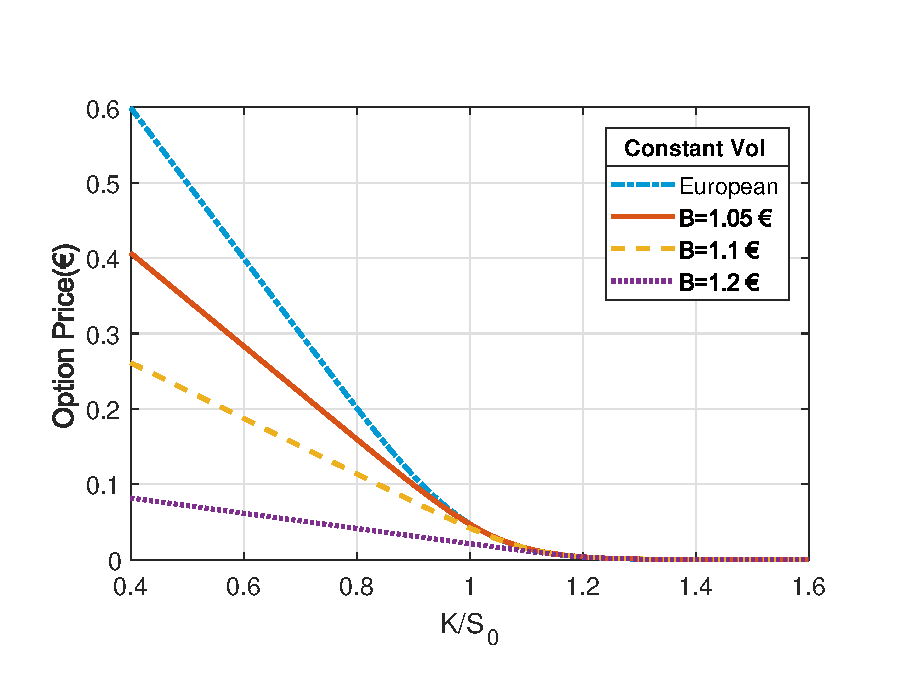
\includegraphics[width=0.49\linewidth,trim={0.5cm 0.4cm 1cm 1cm},clip]{BarrConst}}
    \subfigure[Dupire's Local Volatility model]{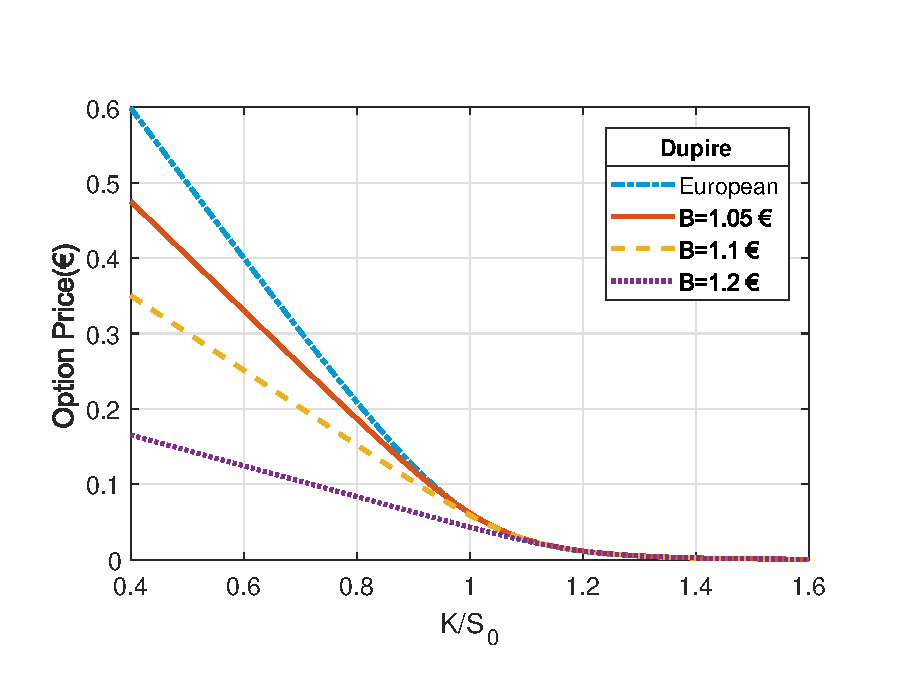
\includegraphics[width=0.49\linewidth,trim={0.5cm 0.4cm 1cm 1cm},clip]{BarrDup}}
        \subfigure[Static SABR model]{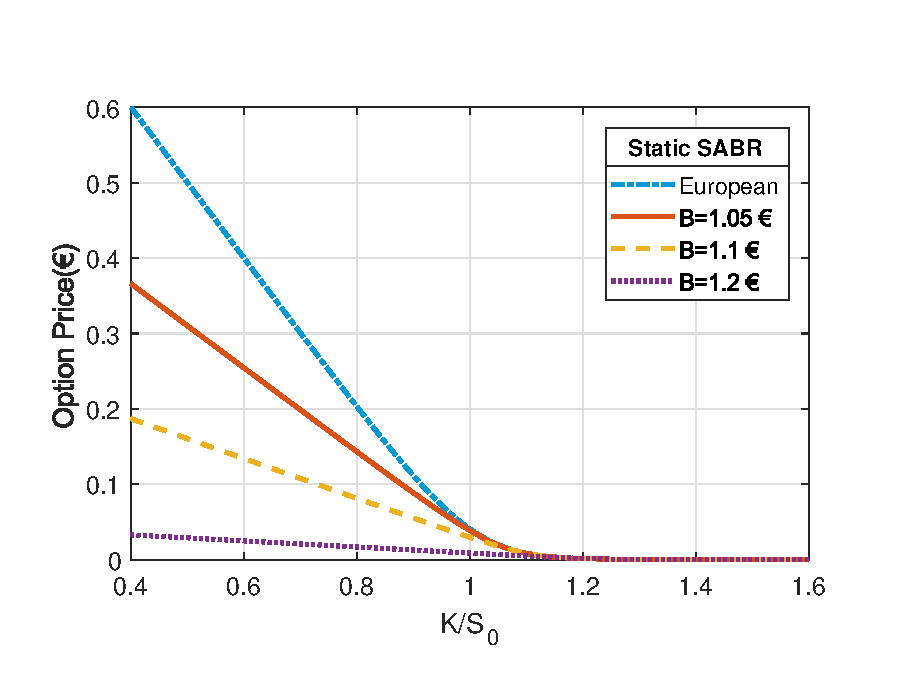
\includegraphics[width=0.49\linewidth,trim={0.5cm 0.4cm 1cm 1cm},clip]{BarrStat}}
            \subfigure[Heston model]{\includegraphics[width=0.49\linewidth,trim={0.5cm 0.4cm 1cm 1cm},clip]{BarrHest}}
                \subfigure[Dynamic SABR model]{\includegraphics[width=0.49\linewidth,trim={0.5cm 0.4cm 1cm 1cm},clip]{BarrDyn}}
  \end{subfigmatrix}
    \caption[Option price curves of simulated European call options and Barrier call options with different barrier levels under each of the models previously studied.]{Option price curves of simulated European call options (light blue dot-dashed lines) and Barrier call options with barrier levels $B=1.05\EUR$ (red full line), $B=1.1\EUR$ (orange dashed line) and $B=1.25\EUR$ (purple dotted line) under each of the models previously studied, for options with a maturity of 42 days.}\label{fig:Barrier}
\end{figure} 

\vfill
\newpage

Analyzing the results of \autoref{fig:Barrier}, we first note that, as expected, when we increase the barrier level the option price decreases. This is indeed observed in all models' simulations, and its cause has been explained before, in \autoref{subsubsection:Barrier Options}.

Possibly the most striking result that we can observe is just how different the price curves are for the simulated barrier options across the models. As an extreme example, we can note that the curve for the Barrier option with barrier level $B=1.1\EUR$ under Dupire's model is actually higher than the curve with barrier level $B=1.05\EUR$ under Heston's model, which should never occur. To explain this phenomenon, we can begin by noting that volatility is particularly important in barrier options. A higher volatility translates into a higher probability of the barrier being surpassed and thus a higher chance of activating the option.
Because each model produces a different volatility behavior, we expect the prices of barrier options to also be very different. Furthermore, we should also note that the models were calibrated on European options. Indeed, when we compare all the European option price curves (blue dot-dashed lines) we can clearly see that they are the same across all models. Thus, we can conclude that even though the models agree when pricing European options (as they should, since they were all calibrated on the same data set), they don't necessarily agree on the prices of Barrier options.

A more in-depth study is required to verify which model produces the most accurate Barrier option prices, but additional data would be required and this study is out of the scope of this work.

\vfill
\newpage

\section{Pitfalls Found in Implementation}
During the implementation of all the models, some pitfalls were found. They were mostly solved, or at least mitigated, and the models were able to perform as expected, as we saw in the previous section. For future reference, and to prevent other researchers from repeating the same mistakes, we now summarize not only the pitfalls observed but also their causes and how we were able to solve them or at least reduce their impact.

\subsection{Dupire Model}
While implementing the Dupire model we noticed that the local volatility surface produced by the model was heavily dependent on the chosen interpolation method. Moreover, we found that it was particularly sensitive to the intervals $\Delta K$ and $\Delta T$ chosen in the interpolation. If chosen to be too large, the gradients wouldn't be able to capture the surface curvature and the local volatility surface would look unrealistic. If chosen to be too small, because we used Delaunay's triangulation method as interpolation, which creates triangular planes between three points, the second derivative would be (wrongly) zero if $K$, $K+\Delta K$ and $K-\Delta K$ were all evaluated inside the same triangular plane, which is bound to be true for the majority of points if $\Delta K$ is small enough.
Thus, the intervals $\Delta K$ and $\Delta T$ have to be chosen very carefully for the model to work properly.

\vfill
\newpage

As an example, in \autoref{fig:DupBad} we show how different choices for $\Delta K$ affect the local volatility surface.



\begin{figure}[H]
  \begin{subfigmatrix}{2}
    \subfigure[Surface Plot, $\Delta K/S_0=0.2$]{\includegraphics[width=0.49\linewidth,trim={1.7cm 0.45cm 1.85cm 0.85cm},clip]{Dup_MS_1.png}}
    \subfigure[Contour Plot, $\Delta K/S_0=0.2$]{\includegraphics[width=0.49\linewidth,trim={0.2cm 0.5cm 1.20cm 1.55cm},clip]{Dup_MS_1C.png}}
        \subfigure[Surface Plot, $\Delta K/S_0=0.025$]{\includegraphics[width=0.49\linewidth,trim={1.7cm 0.45cm 1.85cm 0.85cm},clip]{Dup_MS_2.png}}
    \subfigure[Contour Plot, $\Delta K/S_0=0.025$]{\includegraphics[width=0.49\linewidth,trim={0.2cm 0.5cm 1.20cm 1.55cm},clip]{Dup_MS_2C.png}}
  \end{subfigmatrix}
    \caption[Influence of $\Delta K$ on the local volatility surface.]{Influence of $\Delta K$ on the local volatility surface.}\label{fig:DupBad}
\end{figure} 
 
  
As we can see, both surfaces look highly unrealistic, which serves to demonstrate the severity of choosing inadequate values for $\Delta K$ and $\Delta T$.

There exist two possible alternatives to solve this problem.
On the one hand, we could significantly increase the size of our data set. This would ensure that the size of the triangular planes from Delaunay's triangulation is small enough for the numerical derivatives to produce realistic results, even for small values of $\Delta K$ and $\Delta T$. The problem with this approach is the fact that more data isn't always available, and this alternative may not always  possible.
The other possible path, which was the one implemented, is to test several values for the intervals and observe which of them produces the most realistic gradients and the most realistic local volatility surface. This alternative has the caveat that the choice for the intervals is very subjective and that we lose a great deal of robustness because an interval that is appropriate for a given data set might perform poorly on other data sets.

\vfill
\newpage

\subsection{Heston Model}
In the Heston model, we need to evaluate some integrals to find the closed-form solutions of call prices (eqs. \eqref{P1} and \eqref{P2}).
These integrals are evaluated between $0$ and $\infty$, and, because they are not analytically solvable, they have to be calculated numerically.
We thus obviously need to define some upper limits for the integrals, since numerical integration until $\infty$ is impossible. Cui \textit{et al.}~\citep{Cui} showed that usually these integrals only have to be evaluated until $\approx100$, because the integrands decrease fast enough that they become negligible after this point. During our implementation, this threshold proved to be insufficient when we evaluated the integrals for the earlier maturities with strikes far below and far above $S_0$. For such regions, some erratic oscillating behavior was found, which we represent in \autoref{fig:Hbad}. This behavior was not described by Cui \textit{et al.} possibly because they didn't study the implied volatility curve for such high and low strikes.



\begin{figure}[H]
    \centering
      \includegraphics[width=.65\columnwidth]{HBad.png}
      \caption[Comparison between the different theoretical curves obtained using different values for the upper integration limits in the Heston model.]{Comparison between the different theoretical curves obtained using the values $100$ (green dot-dashed line) and $400$ (red full line) as upper integration limits in the Heston model.}\label{fig:Hbad}
    \end{figure}

This problem was solved simply by increasing the upper integration limits to $400$, for which the oscillating behavior disappeared.



\subsection{SABR Model}
One problem related to the SABR models is the fact that stock prices might become negative, which is clearly absurd. This event is very rare and was usually only found in one of the simulated paths out of $100\,000$.
The reason why this problem only occurred for the SABR models and wasn't observed in Heston is due to the fact that the volatility process in the former is not mean reverting.
This detail enables the volatility process to evolve without restrain. If the volatility process becomes extremely large, the jumps in the stock price process become equally extremely large. In the limit, it is perfectly possible that one of these jumps decreases the stock price process past zero. For the Heston model this problem is not observed because the volatility process (we used the variance process, but they are equivalent) is mean-reverting, so that the volatility doesn't evolve unrestrained and thus the prices don't evolve too erratically.

This negative price shortcoming is more problematic in the SABR model because, in the stock price process, one of the terms is a stock price with an exponent $\beta$. If $\beta\neq\{0,1\}$ and $S(t)<0$, the resulting $S(t+\Delta t)$ will become imaginary, and the whole pricing procedure fails.

To solve this problem, we simply cut the negative stock price paths to zero by applying the function $\max[S(t),0]$, preventing them from becoming negative.



\subsection{Other Problems}
During the implementation we also found that, in the Monte Carlo simulations, updating the volatility process before the stock price produced results that didn't match the theoretical predictions in both the Heston and SABR models.

In other words, if we used
\begin{equation}
S(t+\Delta t)=\sigma(t+\Delta t).\left(\ldots\right)+\ldots,
\end{equation}
instead of the correct
\begin{equation}
S(t+\Delta t)=\sigma(t).\left(\ldots\right)+\ldots,
\end{equation}
\noindent the simulations deviate significantly from the theoretical predictions.
This is expected because the whole correlation mechanism, relating the two stochastic processes through the variable $\rho$, falls apart when we use the first formula.

Though this might seem trivial, some care must be taken when implementing the Monte Carlo pricer to use the updating equations in the correct order.






